\chapter{Method}

This chapter will introduce and develop the \rrtfunnel{} algorithm, by two
means: First develop robust motion primitives through the \ac{SOS} programming
framework based on the work in~\cite{majumdarFunnelLibrariesRealtime2017}, and
second, deploy these funnels as robust motion primitives in a discrete \ac{RRT}
robust motion planner based on~\cite{lavalleLav98cPdf}. Using \textit{robust}
motion primitives has several advantages. Firstly, they are robust to
uncertainty, and thus, as long as the uncertainties in the system are akin to
the assumptions put on the incoming uncertainty parameters, the vehicle will not
leave the funnel, and hence if the funnel is not in collision, neither will the
system be. Secondly, with the assumption that the motion primitives are robust,
there is no need for more conservative maneuvers and heuristics, such as
maximizing the distance to an obstacle. The system might as well choose a
primitive that is close to an obstacle, as one that is far away, as the funnel
is guaranteed to be collision-free in both cases. This means that a robust
motion primitive algorithm can perform more aggressive maneuvers than one that
is inherently conservative about its environment and
maneuvers~\cite{singhRobustOnlineMotion2017}.

\section{Generating robust motion primitives}

In order to create a basic set of funnels as the robust motion primitives for
the \rrtfunnel{} motion planning algorithm, a few obstacles has to be overcome.
The first one is settling on a dynamical system model for the funnel
calculations. This thesis employs the simple unicycle model from
\cite[LaValle.p~613]{Lav06} which is modified slightly into
\begin{equation}
  \label{eq:model-dynamics}
  \mathbf{x} =
  \begin{bmatrix}
    x \\ y \\ \theta \\
  \end{bmatrix}, \, \dot{\mathbf{x}} =
  \begin{bmatrix}
    -v(t)\sin(\theta) \\
    v(t)\cos(\theta) \\
    u \\
  \end{bmatrix},
\end{equation}
which is a first-order unicycle model with constant speed. A picture of the
model can be found in ~\cref{fig:second-order-unicycle}.
\begin{figure}
  \centering { \fontsize{16pt}{16pt}\selectfont \def\svgwidth{1.333in}
    \import{figures/method/}{unicycle-model.pdf_tex} }
  \caption{The unicycle model of a vehicle.}
  \label{fig:second-order-unicycle}
\end{figure}
Although this is the only model used in this thesis, the framework and the code
is easily adapted into accommodating a different and more complicated model.

\subsubsection{Generating the trajectories}

The robust motion primitives are \textit{finite regions of time variance} around
an initial trajectory, meaning that they are all the states surrounding a
trajectory in which the system can reach in a given time interval. But in order
to verify the robust regions surrounding a trajectory, first the trajectories
themselves have to be generated. Generating optimal trajectories is a rich field
in the motion planning literature~\cite{Betts_1998}, and the initial
trajectories could have been generated through any number of methods, however,
the \textit{direct collocation method} was chosen as it builds locally optimal
trajectories from a discrete set of sampled points along a sought trajectory,
which is beneficial for the discrete funnel verification
in~\cref{subsec:generating-funnels}.

The cost function chosen for the solver to minimize is:
\begin{equation}
  J = \int_{0}^{T} \left[ 1 + {u_{0}}^{T}Ru_{0} \right] dt
\end{equation}
from~\cite{majumdarRobustOnlineMotion2013}.

An example of an initial trajectory set is pictured
in~\cref{fig:initial-trajectories}, and consists of a left-turn, a
straight-forward, and a right-turn motion primitive.

\begin{figure}
  \centering
  \begin{minipage}[b]{0.2\textwidth}
    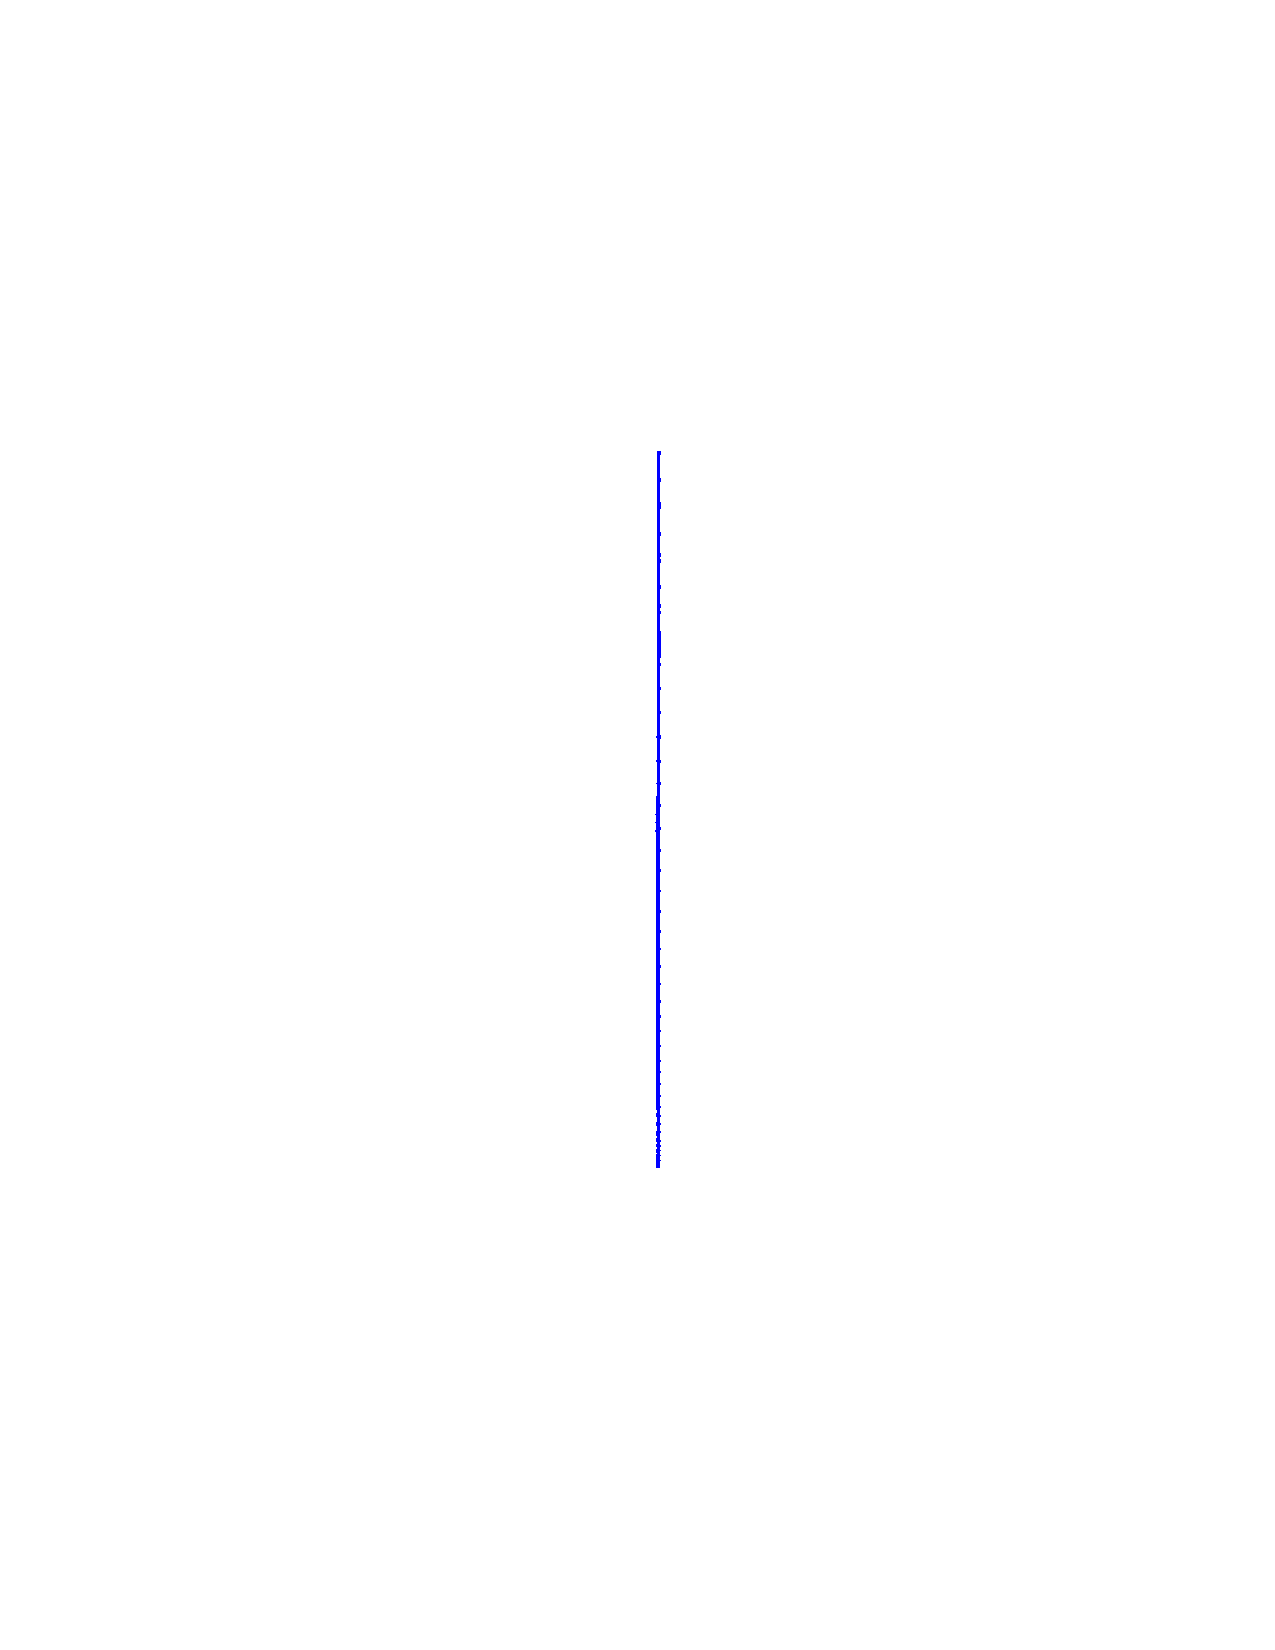
\includegraphics[width=\textwidth]{figures/method/straight-trajector}
  \end{minipage}
  \hfill
  \begin{minipage}[b]{0.2\textwidth}
    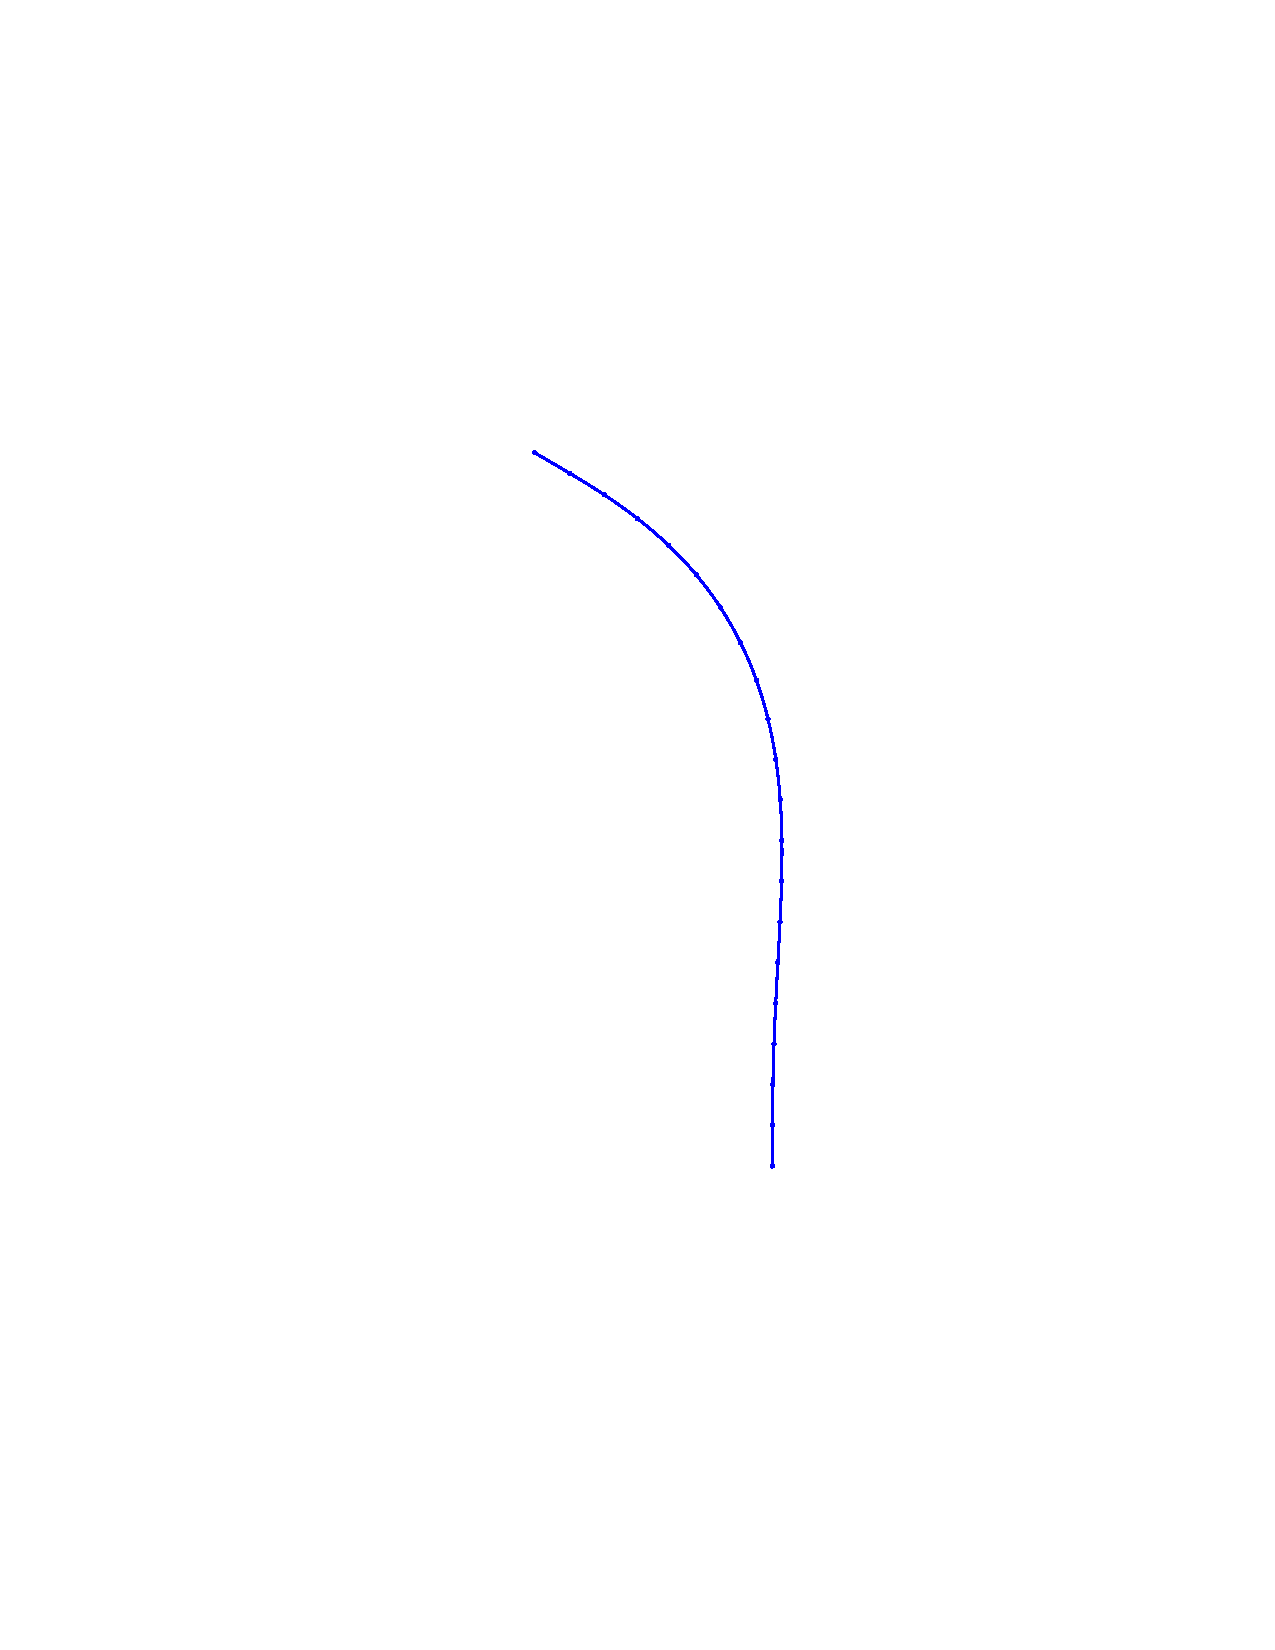
\includegraphics[width=\textwidth]{figures/method/left-trajector}
  \end{minipage}
  \hfill
  \begin{minipage}[b]{0.2\textwidth}
    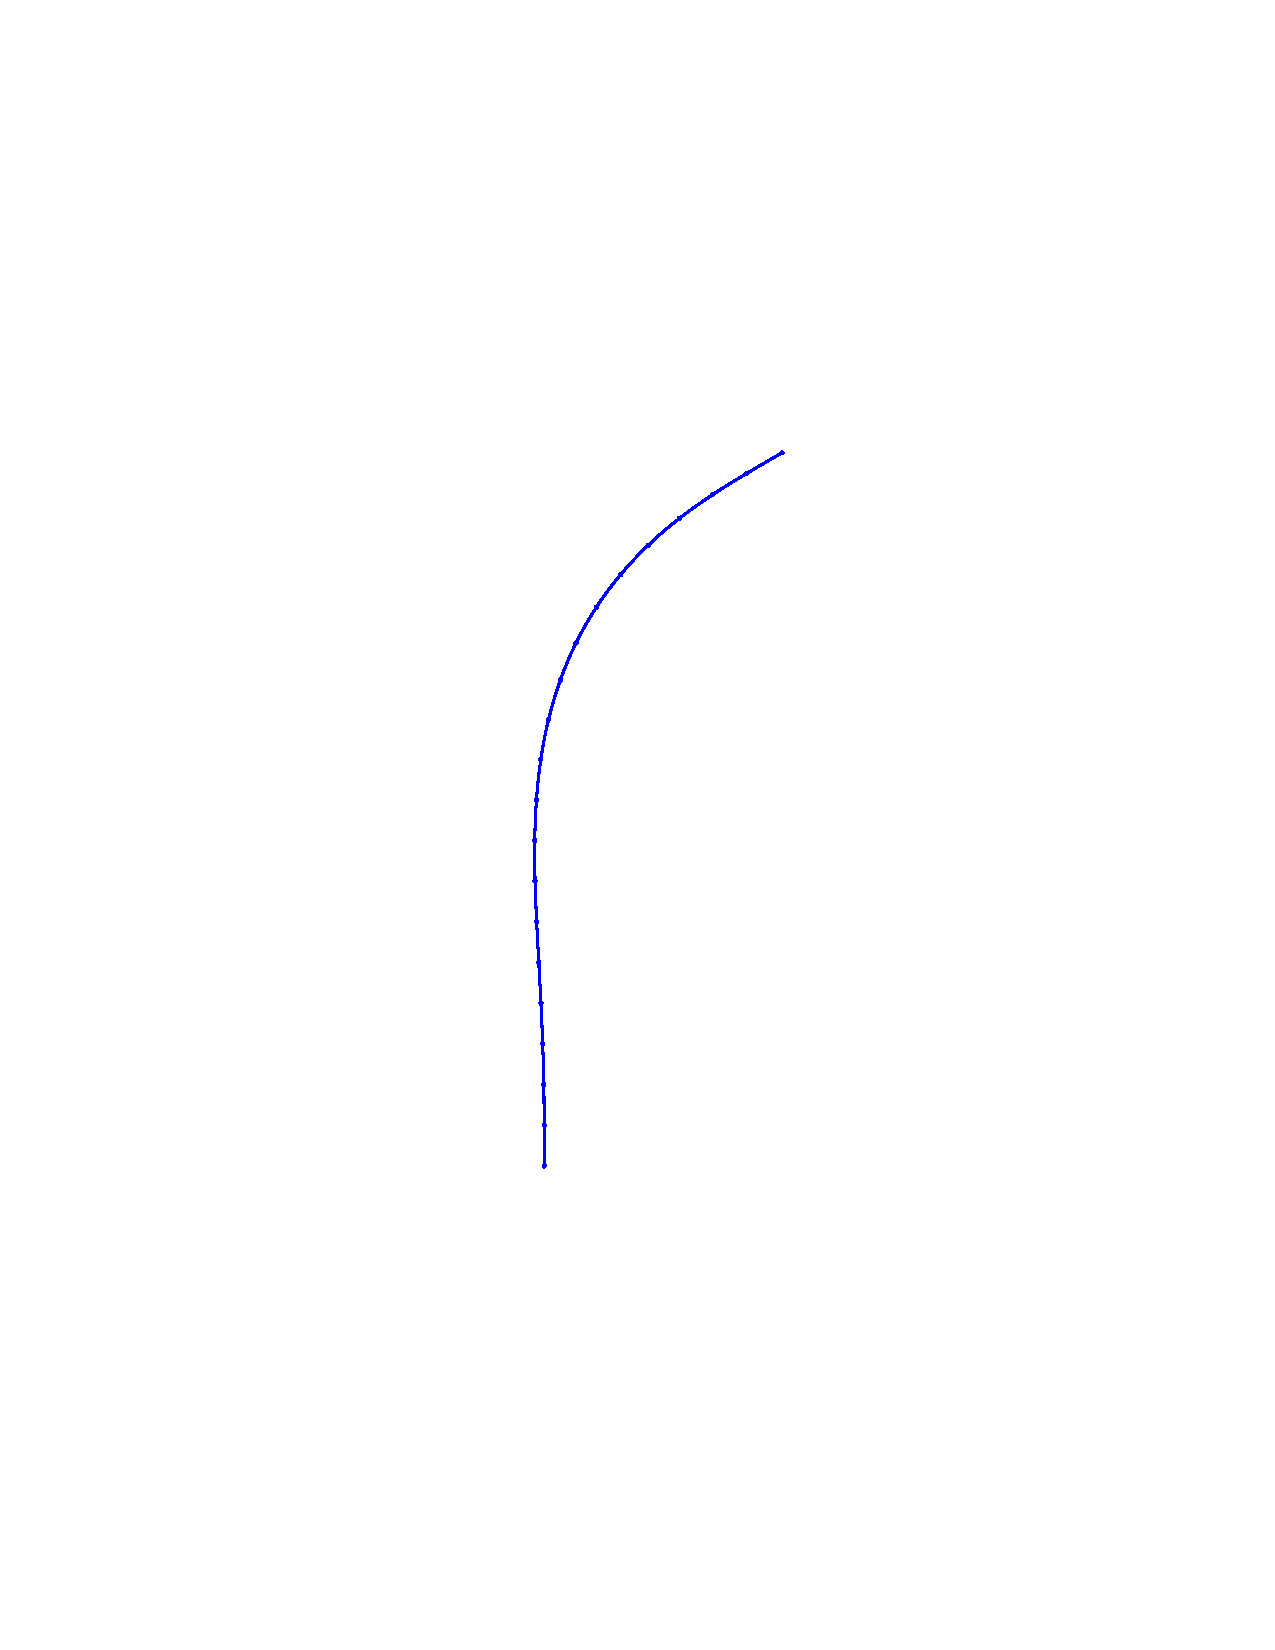
\includegraphics[width=\textwidth]{figures/method/right-trajector}
  \end{minipage}
  \caption{Three motion primitives for the \rrtfunnel{} algorithm, one straight,
    one left, and one right turn.}
  \label{fig:initial-trajectories}
\end{figure}

\subsubsection{Initializing the funnel calculations with a TVLQR candidate as
  the initial Lyapunov function}

The funnel calculation algorithm has to be initialized with a candidate Lyapunov
function. In the same way
as~\cite[Majumdar]{majumdarFunnelLibrariesRealtime2017}, the funnel generation
algorithm will be initialized with a \ac{LQR} controller as the initial Lyapunov
function employing a cost function of the form
\begin{equation}
  J = x^{T}(t_1)F(t_1)x(t_1) + \int_{t_{0}}^{t_{1}} \left( x^{T}Qx + u^{T}Ru + 2x^TNu \right) \mathrm{dt},
\end{equation}
which when employed on the linearization of the system dynamics
\begin{equation}
  \dot{\bar{x}} \approx A(t)\bar{x}(t) + B(t)\bar{u}(t)
\end{equation}
gives an initial candidate Lyapunov function
\begin{equation}
  V(t,x) = {\bar{x}}^{T}S_{i}\bar{x}.
\end{equation}
where \(S_{i}\) is a solution of the \textit{Ricatti} \cref{eq:ricatti}
\begin{equation}
  \label{eq:ricatti}
  - \dot{S}(t) = A^{T}S(t) +S(t)A - \left( S(t)B + N \right)R^{-1}\left( B^{T}S(t) + N^{T} \right) + Q
\end{equation} 
associated with the \ac{LQR} controller.

\subsubsection{Generating the funnels around the trajectories}
\label{subsec:generating-funnels}

With the nominal trajectories, and the initial Lyapunov functions ready, the
funnels around the nominal trajectories can be calculated using the
~\cref{alg:funnelalgorithm}, and is implemented in software through the
~\cite[sostools]{sostools} toolbox.

The dynamics for the model in~\cref{eq:model-dynamics} are still not polynomial,
and the \ac{SOS}-framework can only verify polynomial systems. Thus in order to
obtain the needed polynomial dynamics, the system is expanded around the nominal
trajectory with a Taylor expansion of degree three. Also, the function limiting
the size of the funnel \(\rho(t_{k})\) has to be initialized by a feasible
\(\rho(t)\). This is done through the equation
\begin{equation}
  \rho(t_{k}) = \mathrm{exp}\left( \rho_{\tau}\frac{\left( t_{f} - t \right)}{\left( t_{f} - t_{0}  \right)}\right) + \rho_0
\end{equation}
from~\cite[eq.~6.sec~3]{Tobenkin_2011}, where \(\rho_{\tau}\) is a positive
constant determining the upper bound on the funnel, along with the zero value
\(\rho_0\). If the given choice of \(\rho_{\tau}\) does not verify a funnel,
either increase the value of \(\rho_{\tau}\) and \(\rho_0\), and optionally the
number of sampled points from the trajectory to be
verified~\cite{Tobenkin_2011}.

Thirdly, the initial condition set has to be decided beforehand. In general the
initial condition set can be any semi-algebraic set in the state-space. However,
a simple way of obtaining an initial condition set for the trajectories at hand
is by taking advantage of the Lyapunov function candidate from the
\ac{LQR}-controller. Thus by setting
\begin{equation}
  \mathcal{X}_{0} = \frac{S_{k}}{\rho_{\tau}}
\end{equation}
an initial condition is obtained. In general however, any semi-algebraic set
will do, and the algorithm is not constrained to this one initial condition set
in particular, but it has proven itself useful when calculating new motion
primitives for a system when the initial condition set is not obvious. Another
idea is to use the outlet of one funnel as the initial condition set for the
calculation of another.

The funnels in this thesis are parameterized as sub-level sets of a Lyapunov
function for which the state-space does not invalidate the sub-level constraint.
A visualization of the Lyapunov function associated with a straight motion
primitive can be found in~\cref{fig:visualized-lyapunov}.
\begin{figure}
  \centering
  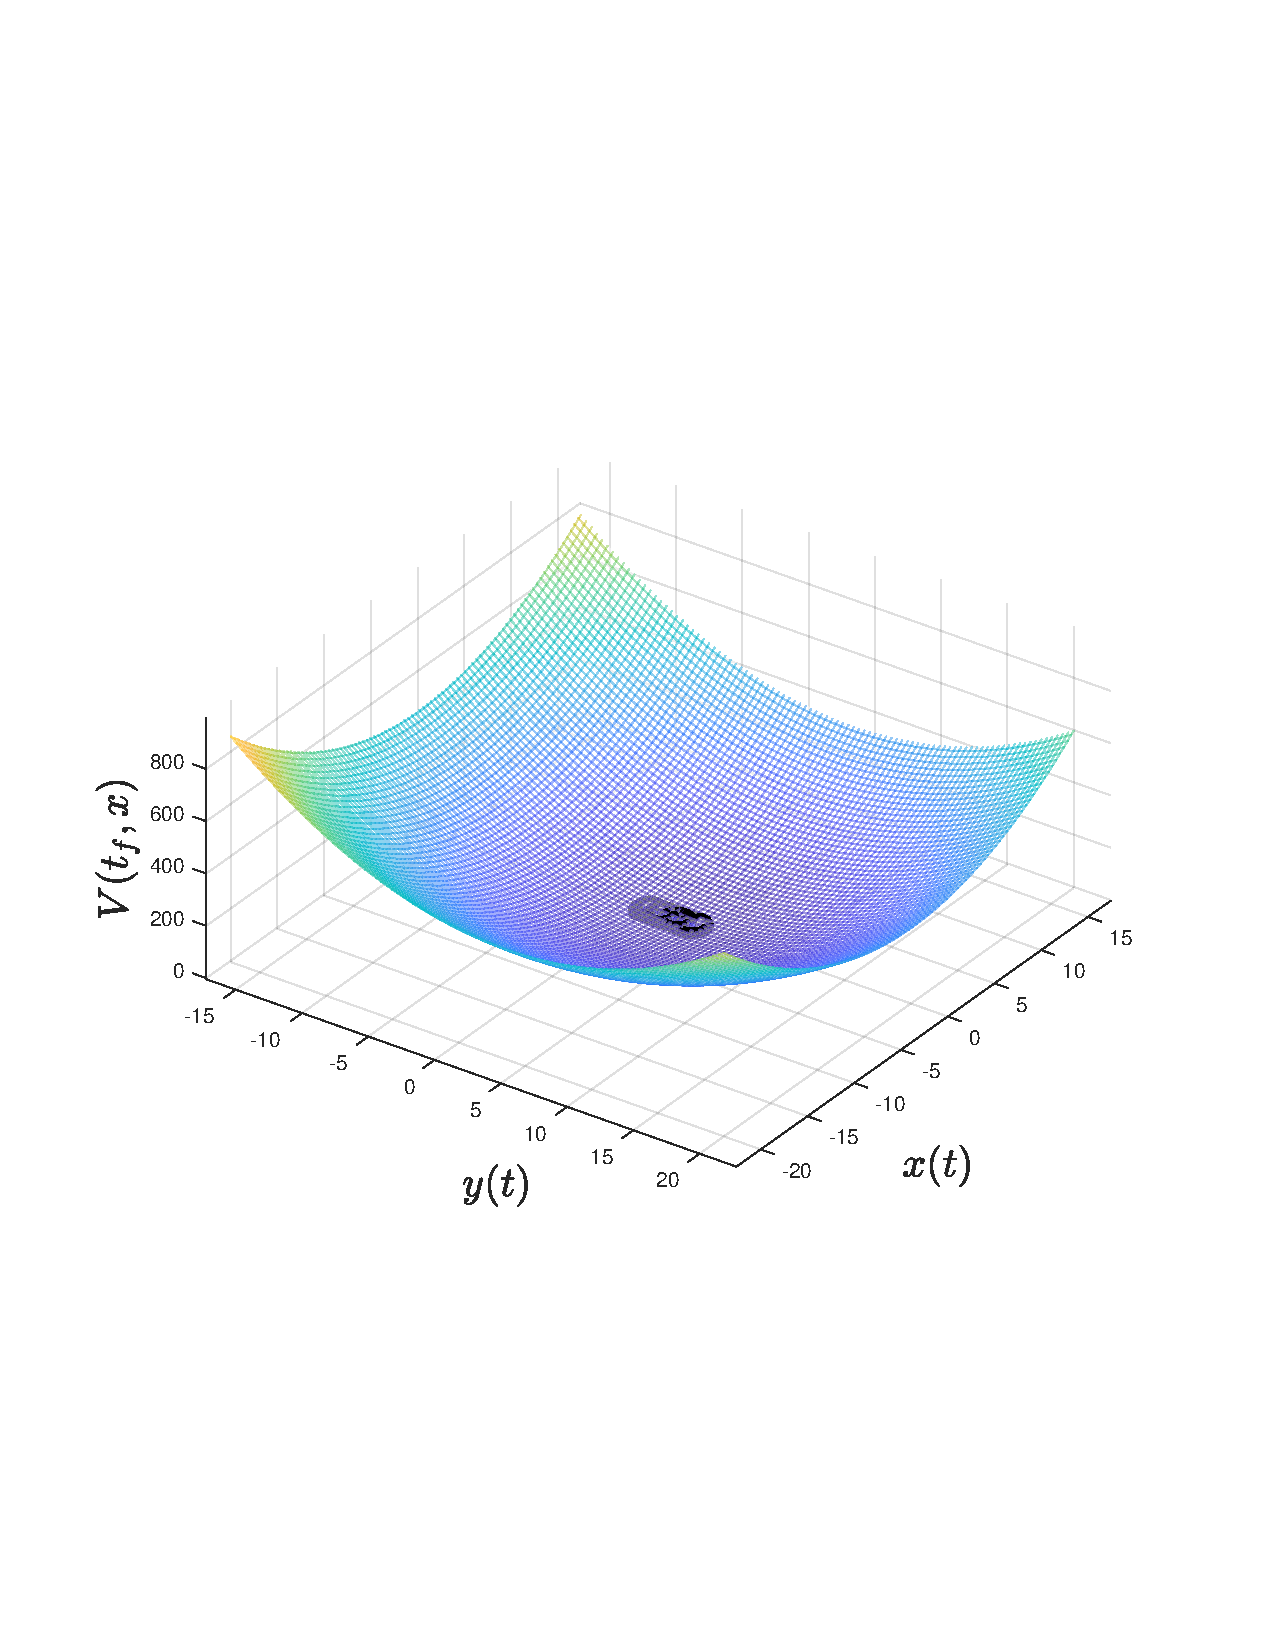
\includegraphics[scale=.3]{figures/rrtfunnel/straight-funnel-lyapunov-3d}
  \caption{A visualization of the Lyapunov function values around a straight
    motion primitive.}
  \label{fig:visualized-lyapunov}
\end{figure}

\subsection{Only minimizing the volume of the funnel projected down into the
  xy-plane}
\label{subsec:xy-cost-function}

In the \rrtfunnel{} algorithm, the size of the of the hyper-ellipsoid which
contains the reachable set is not equally important in all dimensions for all
problems. In the forest traversal case the size of the ellipsoid in the
\(\theta\) dimension is unimportant. There is no need in minimizing the value of
\(\theta\), as it will not make the traversal of the forest any easier, in fact
it might inflate the size of the \((x,y)\) ellipsoid. As an example: For the
vehicle model in this thesis the size of the funnel projected down into the
xy-plane will be the most important metric. Whether or not the vehicle's
orientation parameter \(\theta\) is close to the nominal heading is of less
concern, and is therefore down-prioritized, along with the cost on the control
input \(u\). Having a large \(\theta\) semi-axis in the hyper-ellipsoid can also
be beneficial, as it increases the inlet of the ellipsoid at hand.

For the cost function in the funnel generation
algorithm~\cref{alg:funnelalgorithm}, which in general is a maximization of the
determinant of the upper bound ellipse for the funnel set it is therefore
beneficial to modify this cost to penalize the size of the xy-ellipsoid.

Therefore in order to minimize the actual size of the funnel where the physical
vehicle can move in the world space the cost function has to be modified. Given
a projection map \(\pi : \R^n \rightarrow \R^{n_p}\), the ellipsoid of interest
is \(\mathcal{E} = \set{\bar{x} \in \R^n | \bar{x}^TS_{k}\bar{x} \leq 1}\) with
\[
  S_k^{(p)} = \p{PS_k^{-1}P^T}^{-1}
\]
where \(P\) is an \(n\times n_p\) projection matrix.

Since minimizing the volume of the ellipsoid \(\pi(\mathcal{E})\) using a
\ac{SDP} relies on maximizing the determinant of \(S_k\), and \(det(S_k)\) is a
nonlinear function of \(S_k\), the function has to be linearized in order for it
to be handled by the \ac{SOS} framework.
\cite[Majumdar]{majumdarFunnelLibrariesRealtime2017} solves this by linearizing
\(det(S_k)\) at the solution of \(S_k\) from the previous iteration, and
maximizes this linearization instead. In the end this translates to
\[
  \mathnormal{lin}\p{det\p{S_k}} =
  Tr\p{P^T\p{PS_{k,0}^{-1}P^T}^{-1}PS_{k,0}^{-1}S_kS_{k,0}^{-1}}
\]
where \(S_{k,0}\) is the nominal value for the linearization, and \(Tr\) is the
trace of the matrix.

\subsection{Searching for a controller which minimizes the size of the funnel}

With the non-optimal feedback controller given to the funnel calculation
framework (non-optimal with regards to the funnel calculation cost function),
the size of the funnels will in general be larger than if given a better
controller. Thus in order to further minimize the size of the funnel in the
xy-plane this method, along with the cost function
from~\cref{subsec:xy-cost-function} is used to make traversal through obstacles
in the world space easier. Hence, referring to~\cite[Majumdar.sec~4.3.2
(Feedback control synthesis)]{majumdarFunnelLibrariesRealtime2017}, the initial
controller input to the algorithm can be optimized with the goal of minimizing
the size of the funnel, given a few conditions on the system.

Firstly the system needs to be control affine:
\begin{equation}
  \dot{x} = f(x(t)) + g(x(t))u(t)
\end{equation}
so that the control policy can be parameterized as a polynomial
\(\bar{u}_f(t,\bar{x})\), and the system dynamics written as:
\begin{equation}
  \dot{\bar{x}} = f(x_0(t) + \bar{x}(t)) + g(x(t))\left[ u_0(t) + \bar{u}_f(t,\bar{x}) \right] - \bar{x}_0
\end{equation}
Which~\cref{eq:model-dynamics} is, since:
\begin{equation}
  \dot{x} = %
  f(x(t)) + g(x(t))u(t) = %
  \begin{bmatrix}
    -v(t)\sin (\theta) \\
    v(t) \cos (\theta) \\
    0
  \end{bmatrix}
  +
  \begin{bmatrix}
    0 \\
    0 \\
    1 \\
  \end{bmatrix}
  u(t).
\end{equation}
Then the feedback controller can be optimized by adding the coefficients of the
polynomial \(u_f(t,\bar{x})\) to the set of decision variables in the original
optimization problem. The only issue is that now \(\dot{V}\) is bilinear in the
decision variables \(V\) and \(\bar{u}_f\)
\begin{equation}
  {
    \newcommand{\Vdot}{\dot{V}}
    \Vdot(t,\x) = \frac{\partial V(t,x)}{\partial x} \dot{x} + \frac{\partial V(t,x)}{\partial t}
  }
\end{equation}
Thus in order to minimize the cost function a search is done in
\((\bar{u}_f,\rho,L_t,L_{0,i},S_k)\) while keeping \((V,L,L_{\epsilon,k})\)
fixed. This method combined with the uncertainty added
in~\cref{sec:adding-uncertainty}, is what forms the basis for the funnel
computations as robust motion primitives for traversal in a dense forest
environment, as summarized in~\cref{alg:funnelalgorithm-extended}.

\begin{algorithm}[H]
  \caption{Feedback Funnel computation}
  \label{alg:funnelalgorithm-extended}
  \DontPrintSemicolon \SetAlgoNoLine

  \KwIn{\(V\) and \(\rho\)} \KwOut{Funnel}

  \(cost_{prev} = \infty\)\; converged = false \; \While{\(\not converged\)}{
    Optimization problem 1: \;
    \begin{align*}
      \underset{\substack{\bar{u}_f,L,L_{t},L_{0,i},S_{k},L_{}}}{\inf}&  \sum_{k=1}^{N} \vol(\mathcal{E}(t_{k}))& \\    
      \text{subject to } & V \text{ and } \rho \text{ constant.}& \\
    \end{align*}\;
    Optimization problem 2: \;
    \begin{align*}
      \underset{\substack{\bar{u}}_f,\rho,L_{t},L_{0,i},S_{k}}{\inf}&  \sum_{k=1}^{N} \vol(\mathcal{E}(t_{k}))& \\    
      \text{subject to } & (V,L,L_{\mathcal{E},k}) \text{ constant.}& \\
    \end{align*}\;
    Optimization problem 3: \;
    \begin{align*}
      \underset{\substack{V,\rho, L_{t},L_{0,i},S_{k}}}{\inf}&  \sum_{k=1}^{N} \vol(\mathcal{E}(t_{k}))& \\    
      \text{subject to } & (L,L_{\mathcal{E},k},\bar{u}_f) \text{ constant.}& \\
    \end{align*}\;
    cost = \(\sum_{k=1}^{N} \vol(\mathcal{E}(t_{k}))\) \;
    \If{\(\frac{cost_{prev} - cost}{cost_{prev}} < \epsilon\)} {
      converged = true
    }\;
    \(cost_{prev} = cost\)\;
  }\;
\end{algorithm}


\subsection{Adding uncertainty to the funnel calculation}
\label{sec:adding-uncertainty}

The system dynamics and funnel generation theory presented this far has not been
able to handle any system uncertainty, which is vital to the safe execution of
the \rrtfunnel{} algorithm. However, the basic formulations presented do have
all the necessary formulations present, and adding uncertainty is equivalent to
adding another constraint to the optimization
problem~\cref{opt:sufficient-conditions}.

Following are the changes to the formulation of the \ac{SOS} optimization
condition~\cref{eq:funnelsufficient} from~\cite{majumdarRobustOnlineMotion2013}
so that a funnel takes into account a bounded uncertainty term of the form
\(\mathcal{W} = \set{ w(t) \in R^d \mid g_{w,j}(w) \geq 0\, \forall j =
  1,\ldots,N_w}\). But first the uncertainty has to be added to the system
dynamics equation. This is done through adding an uncertainty term \(w\)
\begin{equation}
  \dot{\bar{x}} = f_{cl}(t, \bar{x}(t), w(t)).
\end{equation}
Which in this thesis is an added uncertainty to~\cref{eq:model-dynamics} so that
\begin{equation}
  \dot{\bar{x}} = %
  \begin{bmatrix}
    -v(t)\sin(\theta) \\
    v(t)\cos(\theta) \\
    -Kx(t) \\
  \end{bmatrix}
  +
  \begin{bmatrix}
    w(t) \\
    0 \\
    0
  \end{bmatrix}.
\end{equation}
Then the requirement~\cref{eq:reachableset} is slightly modified so that
\begin{equation}
  \label{eq:uncertain-reachableset}
  \bar{x}(0) \in \mathcal{X} \implies \bar{x}(t) \in F(t),\, \forall t \in
  [0,T], \, \forall w \colon [0,T] \rightarrow \mathcal{W}
\end{equation} 
where \(F(t)\) is the new reachable set for the uncertain system. Thus the
sufficient condition~\cref{eq:funnelsufficient} turns into
\begin{equation}
  \label{eq:funneluncertain-sufficient}
  V(t,\bar{x}) = \rho(t) \implies \dot{V}(t,\bar{x},w) < \dot{\rho}(t), \, \forall t \in [0,T], \, \forall w(t) \in \mathcal{W}.
\end{equation}
The Lyapunov function derivative then becomes
\begin{equation}
  \dot{V}(t,\bar{x}, w) = \frac{\partial V(t,\bar{x})}{\partial x} f_{cl}(t,\bar{x},w) + \frac{\partial V(t,\bar{x})}{\partial t},
\end{equation}
and the optimization condition~\cref{eq:sufficient-conditions} turns into
\begin{align}
  \label{eq:optimizationconditionuncertain}
  \dot{\rho}(t) - \dot{V}(t,\bar{x},w) - L(t,\bar{x},w) \left[ V(t,\bar{x}) - \rho(t) \right] - L_{t}(t,\bar{x},w)\left[ t\left( T - t \right) \right]  & \nonumber \\
  - \sum_{j=1}^{N_{w}} L_{w,j}(t,\bar{x},w)g_{w,j}(w) \quad \text{is SOS} &  \\
  L_{w,j}(t,\bar{x},w) \qquad \text{is SOS}, \; \forall j = 1,\ldots,N_w \nonumber
\end{align}

\subsubsection{Shifting funnels and invariance}

Now that the funnels are able to be calculated for a basic set of motion
primitives, it is time to start looking at chaining these primitives together in
order to construct longer and more complex motions from a basis set of motion
primitives. Thus, in order to freely shift funnels around in the configuration
space, the cyclic coordinates of the system has to be determined, so that the
dynamics of the system is never violated. Even though the funnels now start and
end in a completely different part of the configuration space, the original
dynamics must not be violated. Therefore the cyclic and non-cyclic coordinates
of the system must be decided~\cref{subsec:cyclic-coordinates}. Therefore, given
the model~\cref{eq:model-dynamics} the cyclic coordinates of the system are
found from:
\begin{align*}
  \mathcal{L} &= T - V = \frac{1}{2} mv^2 + \frac{1}{2}I\dot{\theta}^2 \\ 
              &= m \left(
                v^2 \sin^2 \theta + v^2 \cos^2 \theta
                \right)  + I {\dot{\theta}}^2 \\
              &= mv^2 + I {\dot{\theta}}^2 \\
\end{align*}
which shows that the Lagrangian is invariant to shifts in the \((x,y,\theta)\)
variables, since \(\frac{\partial\mathcal{L}}{\partial q_i} = 0 \, q_i =
x,y,\theta\). Now, any funnel in the base set can be shifted freely around in
the cyclic coordinates of the system without changing the solution to the system
dynamic equation, and thus create an infinite set of funnels in the state space
for the planner to work with. Through the partitioning of coordinates into
cyclic- and non-cyclic coordinates of the form \(x = [x_c\, x_{nc}]\), the state
dynamics \(\dot{x} = f(x(t), u(t))\) only depends on the non-cyclic coordinates
of the system. Thus, a trajectory of the form \(t \rightarrow (x(t),u(t))\)
which solves \(\dot{x} = f(x(t),u(t))\) can then be transformed through a shift
\(\Psi_c\) along the cyclic coordinates of the system to yield a valid solution
of the form
\[
  t \rightarrow (\Psi_{x}(x(t)), u(t))
\]
where the transform \(\Psi\) is given by
\[
  \Psi([x_c, x_{nc}]) =
  \begin{cases}
    x_c \rightarrow \hat{x}_{c} \\
    x_{nc} \rightarrow x_{nc} \\
  \end{cases}.
\]

\subsection{Sequential funnel composition}
\label{sec:composable-funnels}

Now that funnels can be shifted freely around the configuration space along the
cyclic coordinates of the system to create new motion primitives it is time to
start chaining funnels together to create trees of funnels that span out into
the planning environment in order to create a robust motion plan. However, in
order for two funnels to create a third and new motion primitive when chained
together they need to be composable, which means that the inlet of the second
funnel needs to be fully contained within the outlet of the first one. Otherwise
the robustness guarantees of the traversal will be lost. An abstract pictorial
representation of two funnels composed together can be seen
in~\cref{fig:two-funnels-composed} to emphasize this observation. The
mathematical definition of funnel composition~\cref{def:funnel-composition} that
is used to verify that two funnels are composable, and is implemented as a
\ac{SOS}-program in~\cref{AppendixB}. However, take note that the definition has
to be modified slightly in order to take into account the translation along the
cyclic coordinates of the system. Hence the definition used
is~\cite[definition~3,sec~5]{majumdarFunnelLibrariesRealtime2017} which states
\begin{definition}
  An ordered pair \(F_1,F_2\) of funnels \(F_1 \colon [0,T_1] \rightarrow
  \mathcal{P}(\R^n)\) and \(F_2 \colon [0,T_2] \rightarrow \mathcal{P}(\R^n)\)
  is \textit{sequentially composable modulo invariance} if there exists a shift
  along cyclic coordinates such that \(F_{1}(T_1) \subset
  \Psi_{c}\left(F_2(0)\right)\)
\end{definition}
In layman's terms this means that if a funnel \(F_2\) can be shifted along
cyclic coordinates to stack up against the outlet of funnel \(F_2\) so that they
are composable in the sense of definition~\cref{def:funnel-composition}, they
are composable modulo invariance. Hence, any funnel in the configuration space
will be a set consisting of the funnel from the basic set, along with a
transformation along the cyclic coordinates of the system \(\hat{\mathcal{F}} =
\set{F_n \in \R^n \mid \Psi_{c,i}(F_i), F_i \in \mathcal{F}}\), where
\(\mathcal{F}\) is the basic set of funnels.

\begin{figure}
  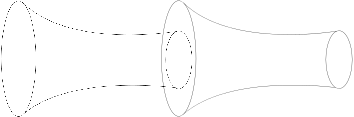
\includegraphics[scale=.2]{figures/method/funnel-composition} \centering
  \caption{Two funnels that can be successfully composed, as the outlet of the
    first one is fully contained in the inlet of the second.}
  \label{fig:two-funnels-composed}
\end{figure}

Using the generalized S-procedure
\begin{equation}
  V_1(T_1,\bar{x}) \leq \rho_1(T_1) \implies V_2(0, \bar{x}) \leq \rho_2(0)
\end{equation}
the composability of two funnels can be checked through the \ac{SOS} program
\begin{align}
  & \text{Find } && L(\bar{x}) \\
  & \text{s.t. } && \rho_2(0) - V_2(0,\bar{x}) - L(\bar{x})\left( \rho_1(T_1) - V_1(T_1,\bar{x}) \right) \text{ is SOS} \nonumber \\ 
  &&& L(\bar{x}) \text{ is SOS} \nonumber
\end{align}
A picture of funnels composed together can be seen
in~\cref{fig:funnel-composition-tree}.
\begin{figure}
  \centering 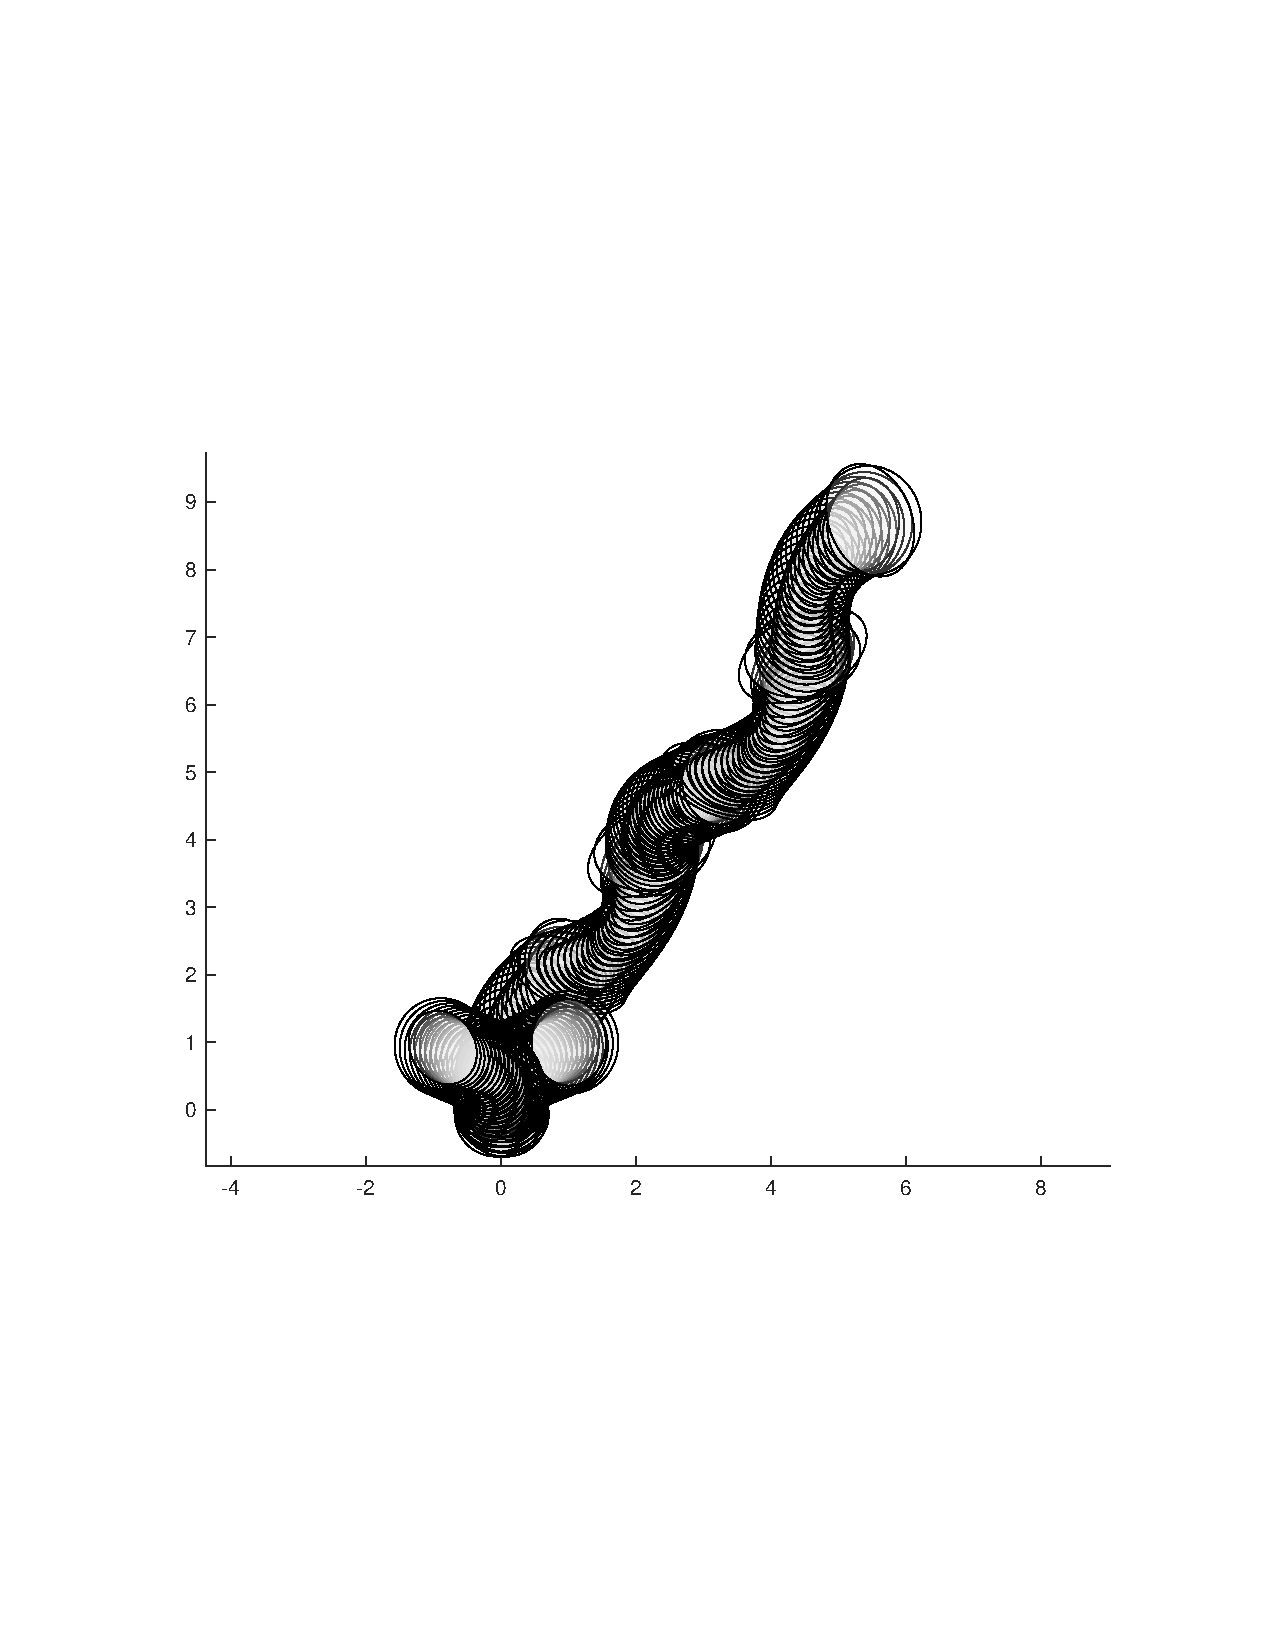
\includegraphics[scale=.5]{figures/method/funnel-tree}
  \caption{Pictured: A tree of funnels built by the \rrtfunnel{} algorithm,
    showing how longer motion primitives are built up from primitives in the
    basic set.}
  \label{fig:funnel-composition-tree}
\end{figure}

\subsection{Checking the conservativeness of the funnel calculated}

The funnels generated are \textit{outer approximations} of time reachable sets
for the system at hand. This means that in general they are larger than the
actual reachable set for the system. This can be verified through a Monte-Carlo
simulation for the straight funnel primitive. Therefore, running N-simulations
from the funnel inlet, and storing the solutions, it is possible to visualize
the actual funnel for the system. An example of which can be seen
in~\cref{fig:funnel-simulated-overlaid}.

By comparing one of the funnels in the funnel set with a funnel based from
\(10.000\) simulation runs, it is seen that the calculated funnels are indeed
proper outer approximations of the time-reachable sets for the dynamical system.
Therefore, the conclusion is that the uncertain trajectories are contained
within the funnels used in the planner, and the trajectories can be seen as
robustly to uncertainty given the uncertainty and dynamical assumptions made.

\begin{figure}
  \begin{subfigure}[b]{0.3\textwidth}
    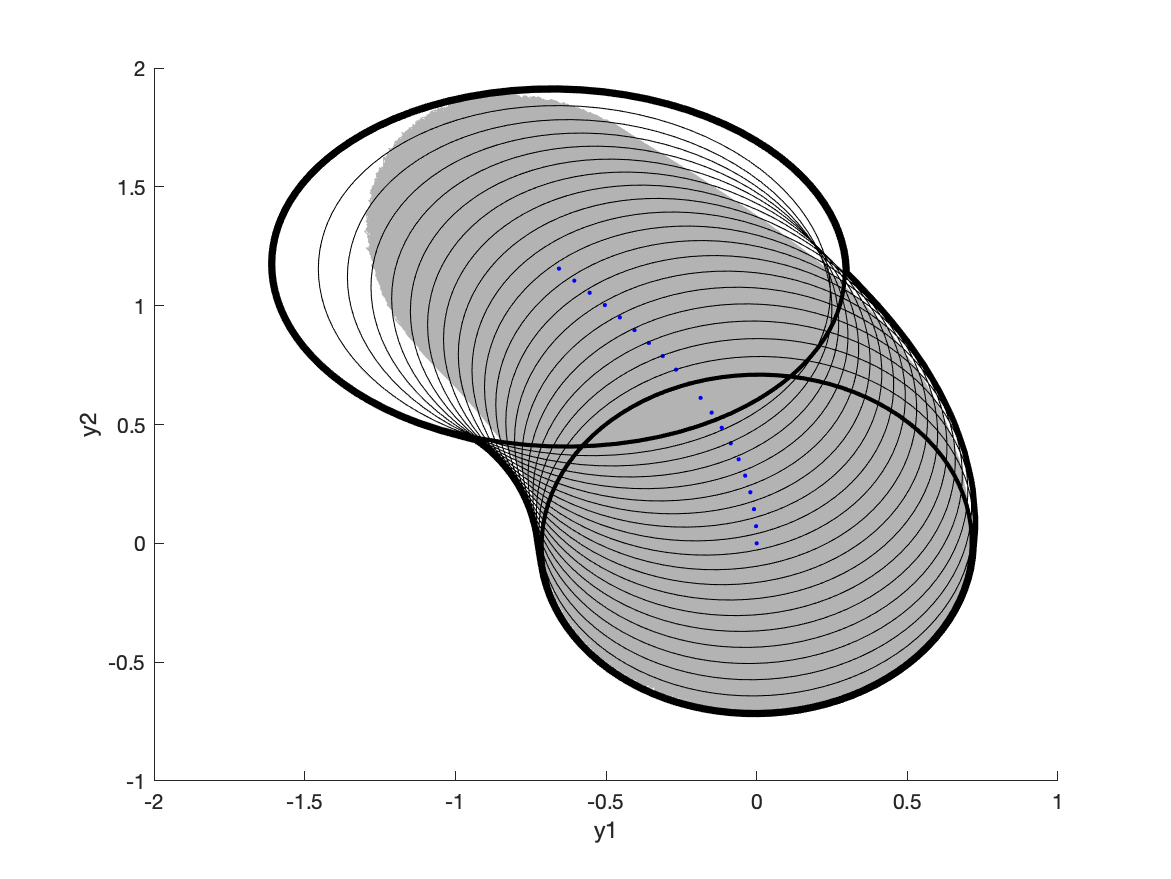
\includegraphics[width=\textwidth]{figures/experiments/FunnelSim4}
  \end{subfigure}
  % add desired spacing between images, e. g. ~, \quad, \qquad, \hfill etc.
  % (or a blank line to force the sub-figure onto a new line)
  \begin{subfigure}[b]{0.3\textwidth}
    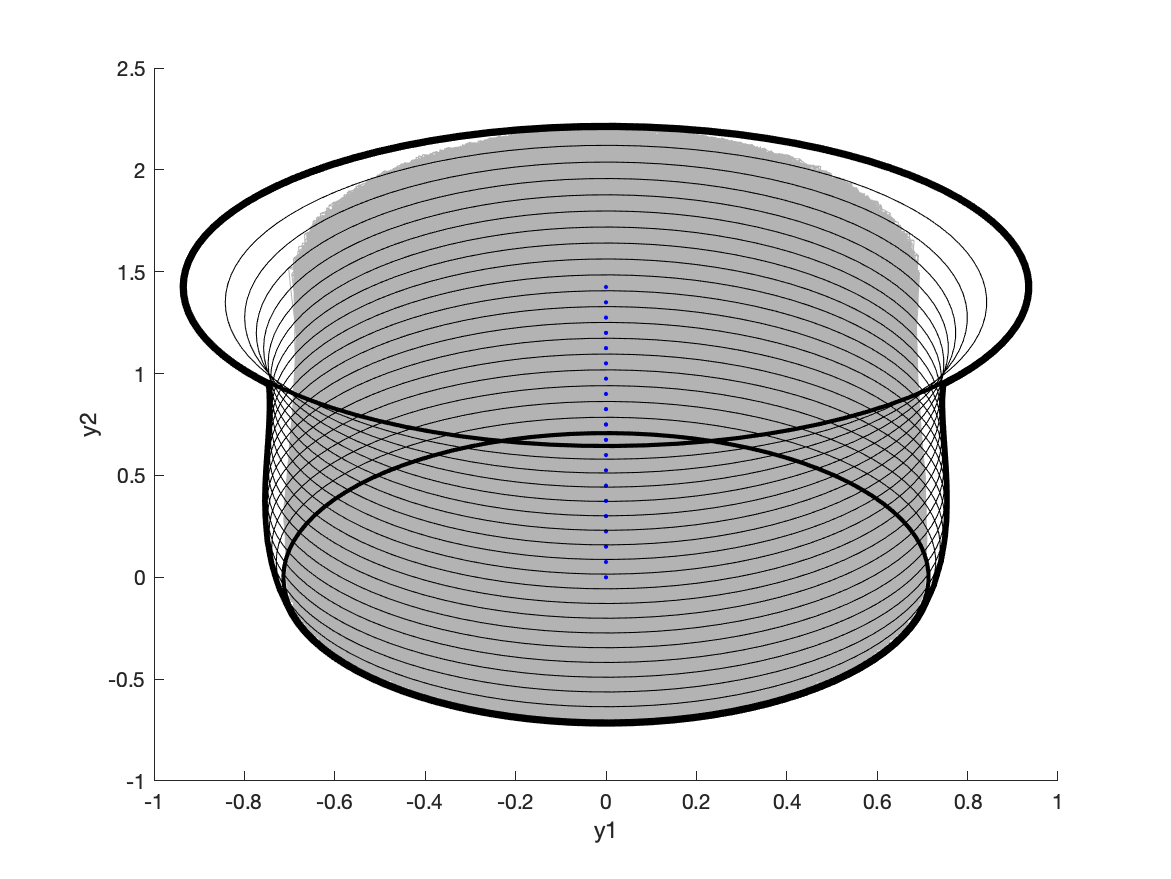
\includegraphics[width=\textwidth]{figures/experiments/FunnelSim1}
  \end{subfigure}
  \begin{subfigure}[b]{0.3\textwidth}
    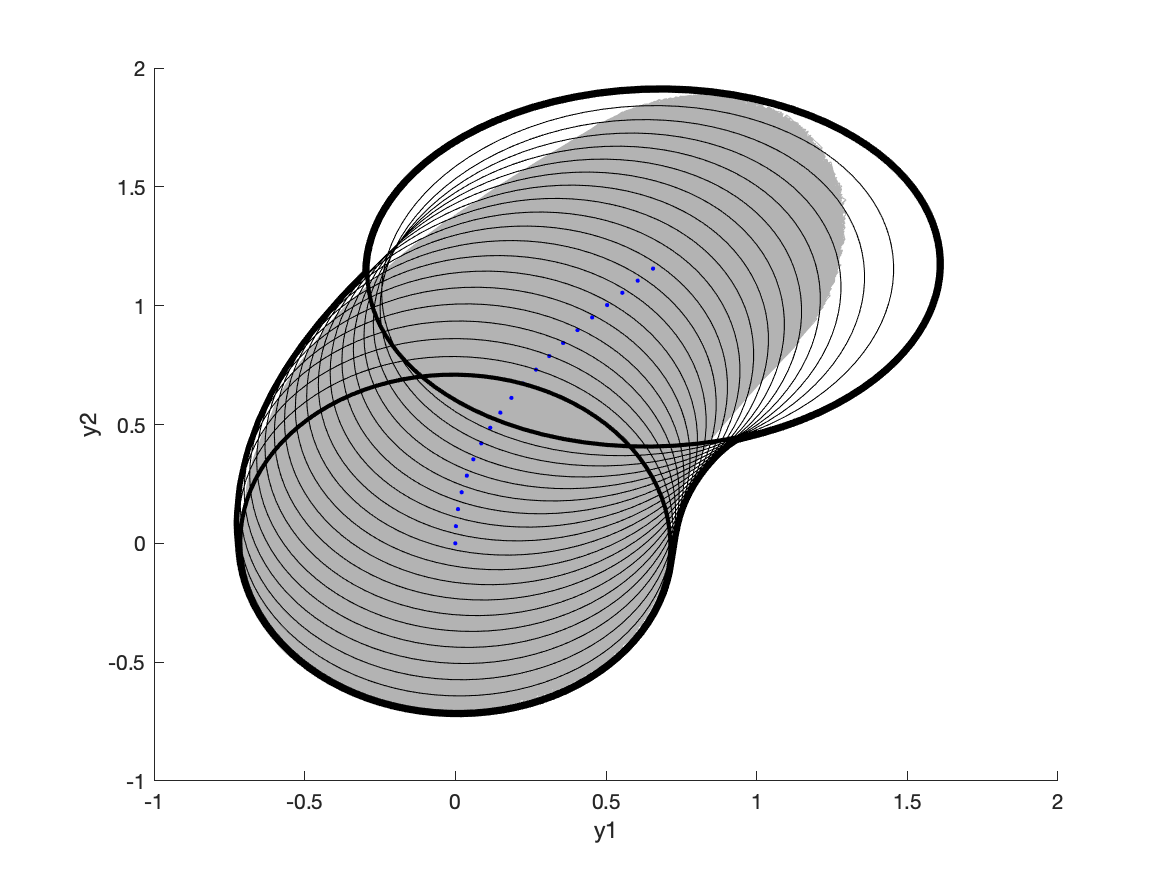
\includegraphics[width=\textwidth]{figures/experiments/FunnelSim5}
  \end{subfigure}
  % add desired spacing between images, e. g. ~, \quad, \qquad, \hfill etc.
  % (or a blank line to force the sub-figure onto a new line)
  \caption{The simulated trajectories, overlaid with the outer approximation
    that is the funnel returned by the \ac{SOS} calculation for three
    trajectories from the trajectory library \(\mathcal{T}\).}
  \label{fig:funnel-simulated-overlaid}
\end{figure}

\begin{figure}[p]
  % Regular xy-funnel
  \begin{minipage}{0.5\textwidth}
    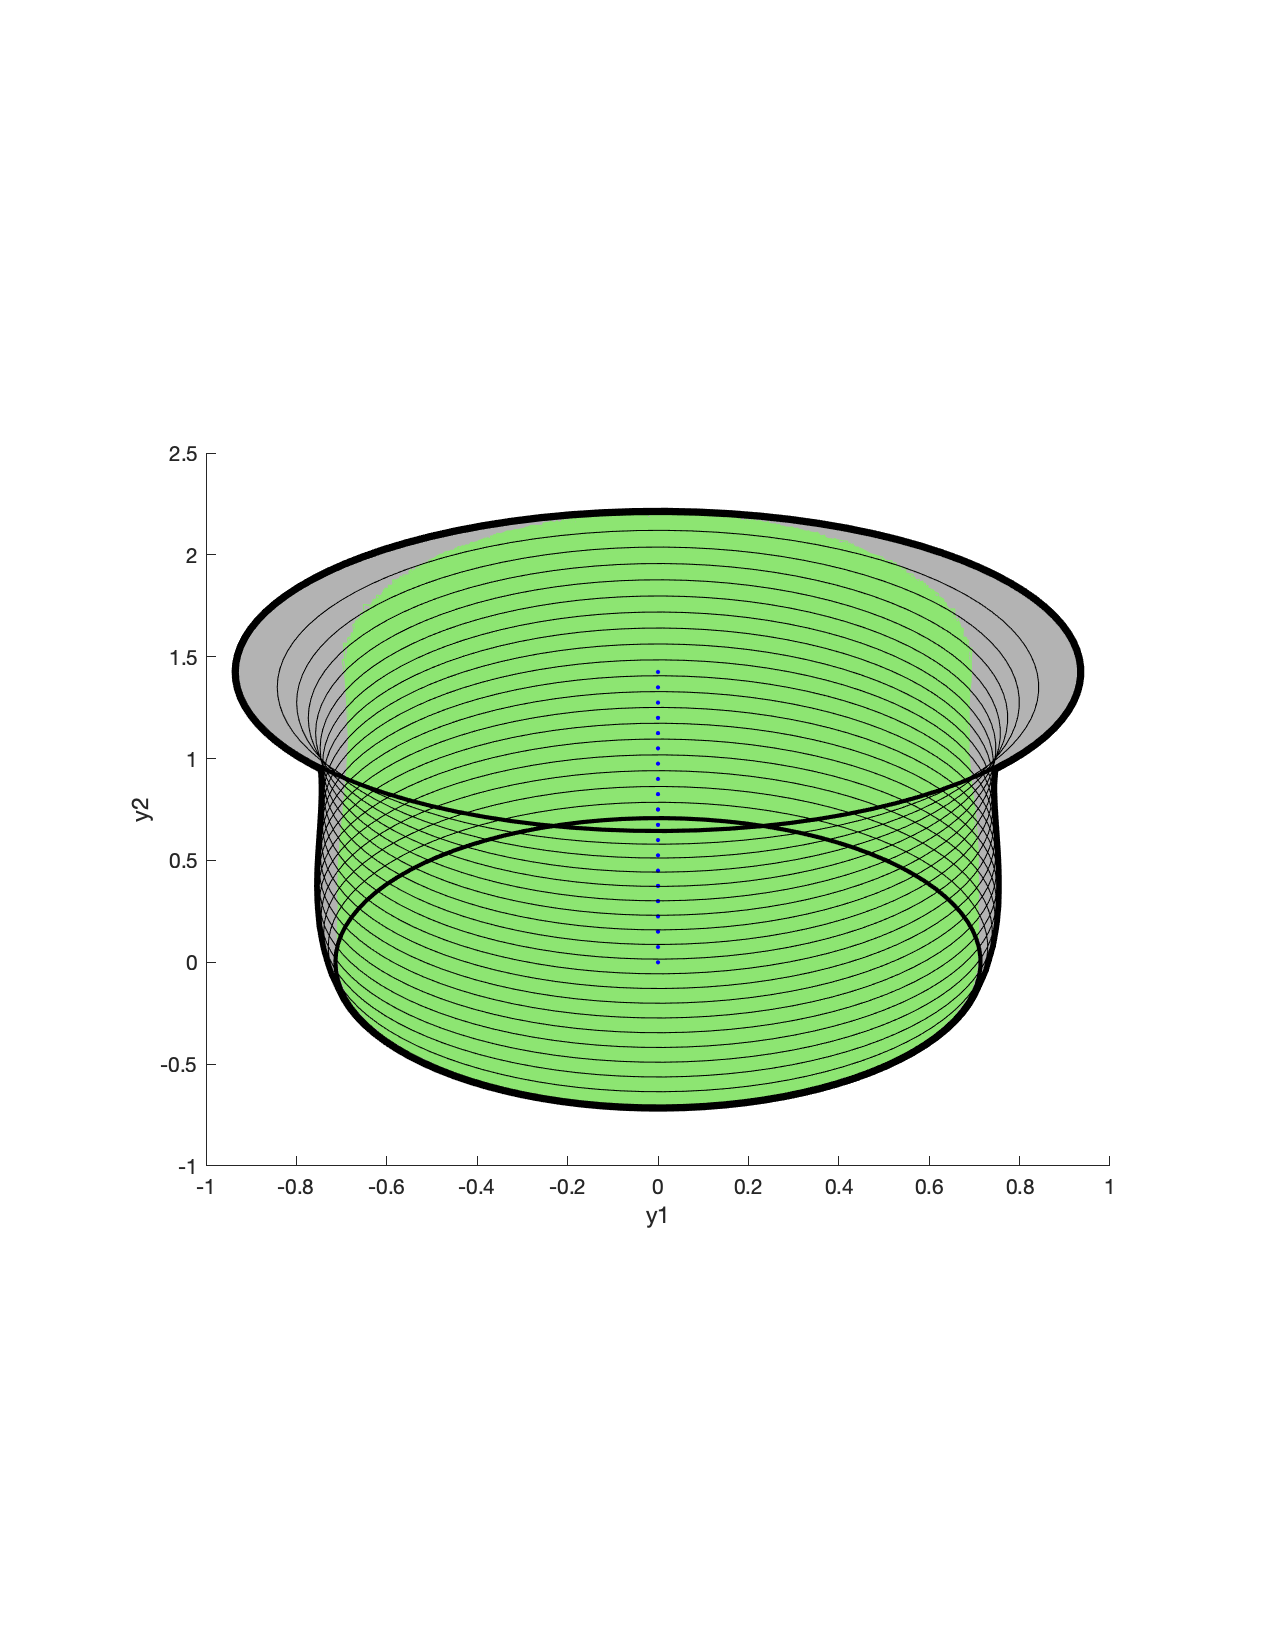
\includegraphics[width=\textwidth]{figures/method/FunnelSim1}
    \caption{Comparison of the \ac{SOS} funnel in the xy-plane with the
      simulated non-polynomial system overlaid in green, generated from
      \(10.000\) Monte-Carlo simulations.}
  \end{minipage}%
  % 
  \begin{minipage}{0.5\textwidth}
    % y-theta funnel
    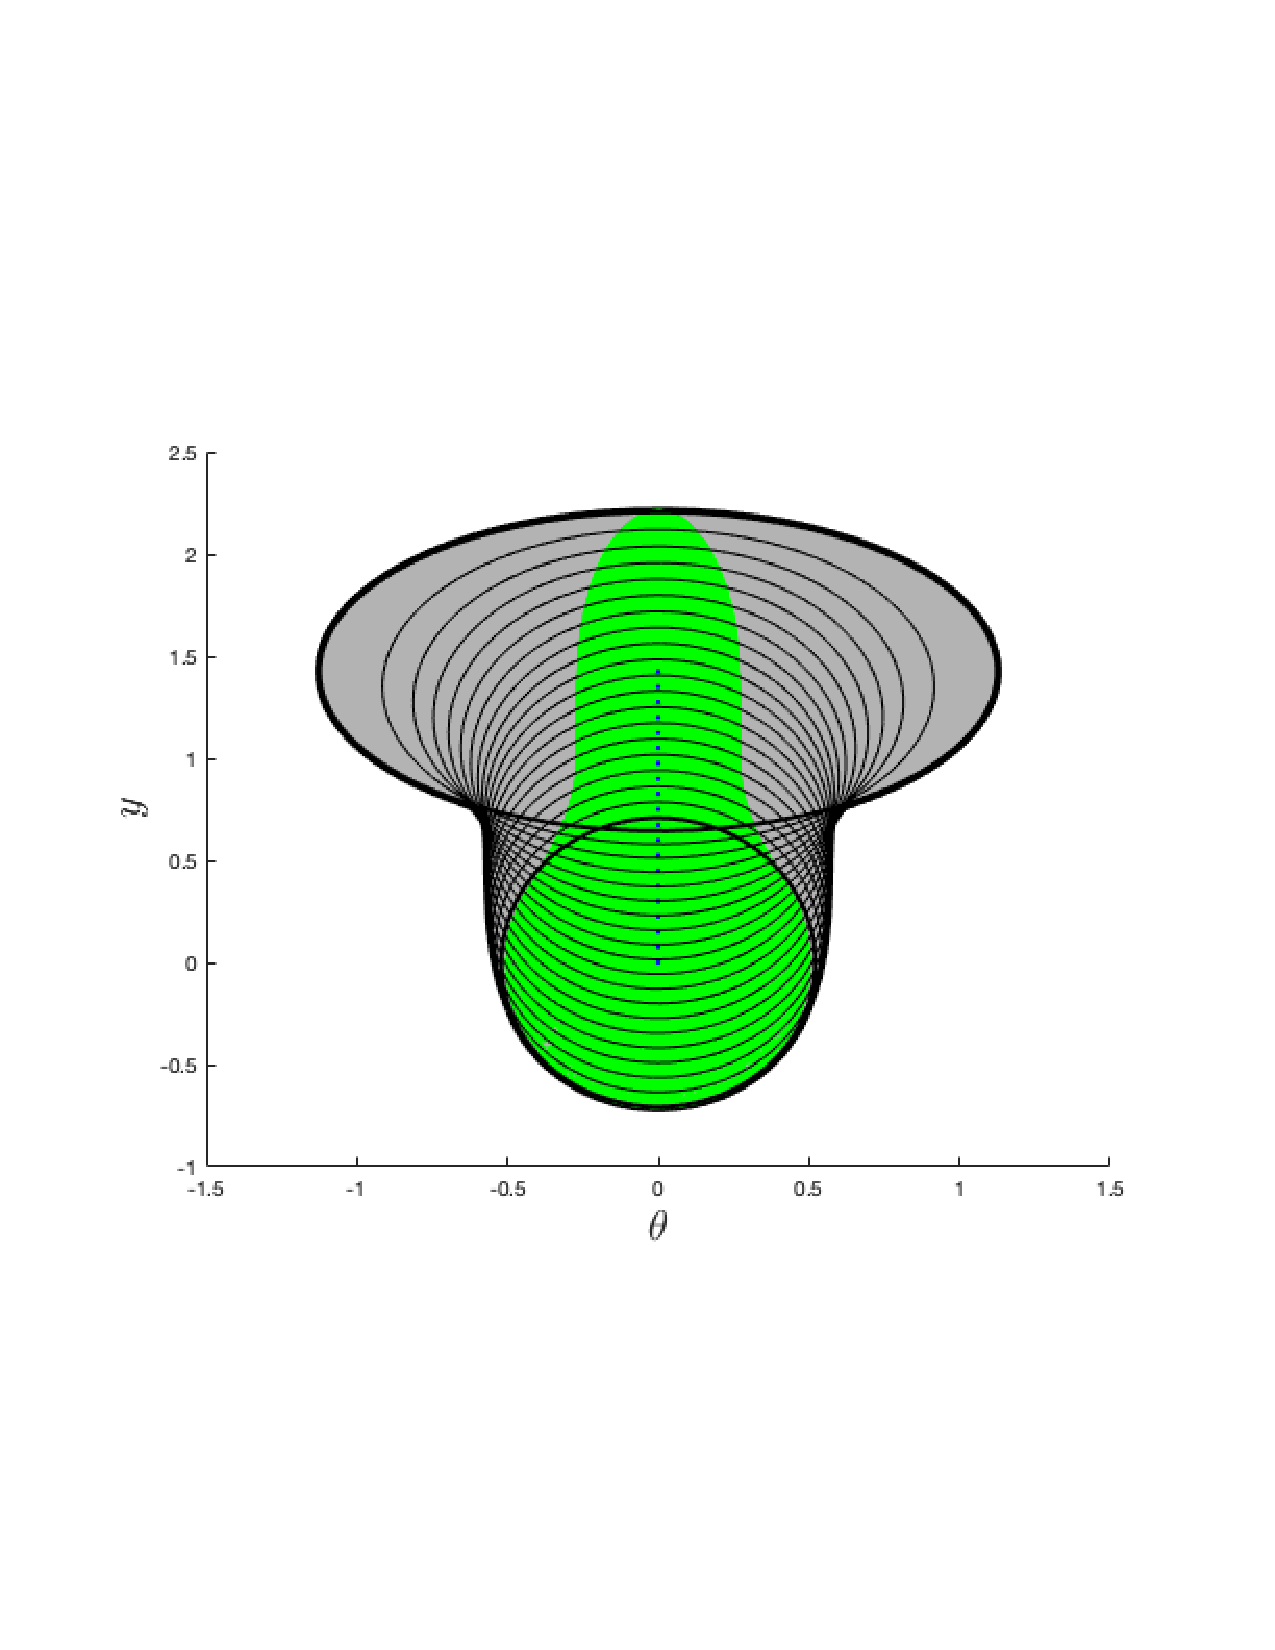
\includegraphics[width=\textwidth]{figures/method/FunnelSimythetafunnel}
    \caption{Comparison of the \ac{SOS} funnel in the \(\theta\)-y plane, with
      the simulated non-polynomial system overlaid in green, generated from
      \(10.000\) Monte-Carlo simulations.}
  \end{minipage}%
  % 
  \\
  %
  \fbox{%
    \begin{minipage}{0.5\textwidth} % Left subfig
      % 
      \begin{minipage}[b]{0.5\textwidth} % Inner left
        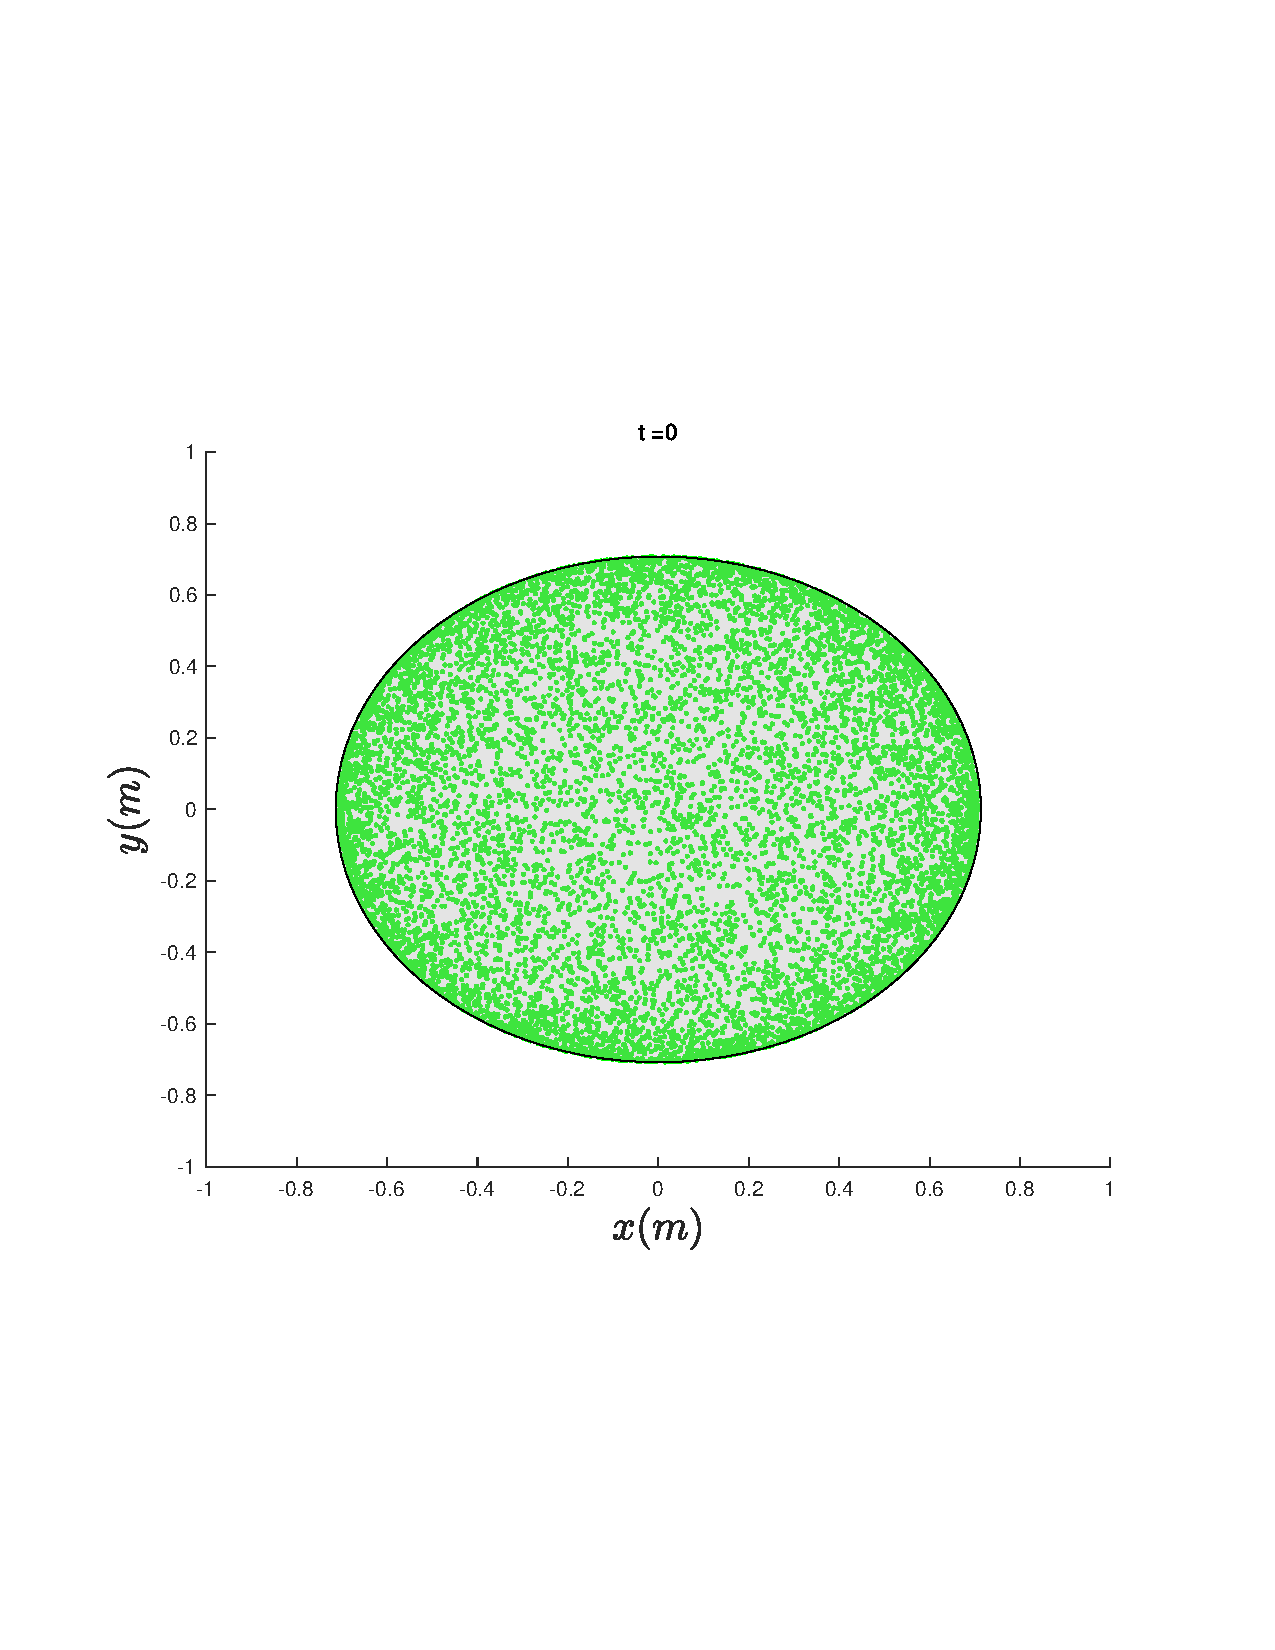
\includegraphics[width=\textwidth]{figures/method/FunnelSimOverlaid1funnel-1}
      \end{minipage}%
      % 
      \begin{minipage}[b]{0.5\textwidth}
        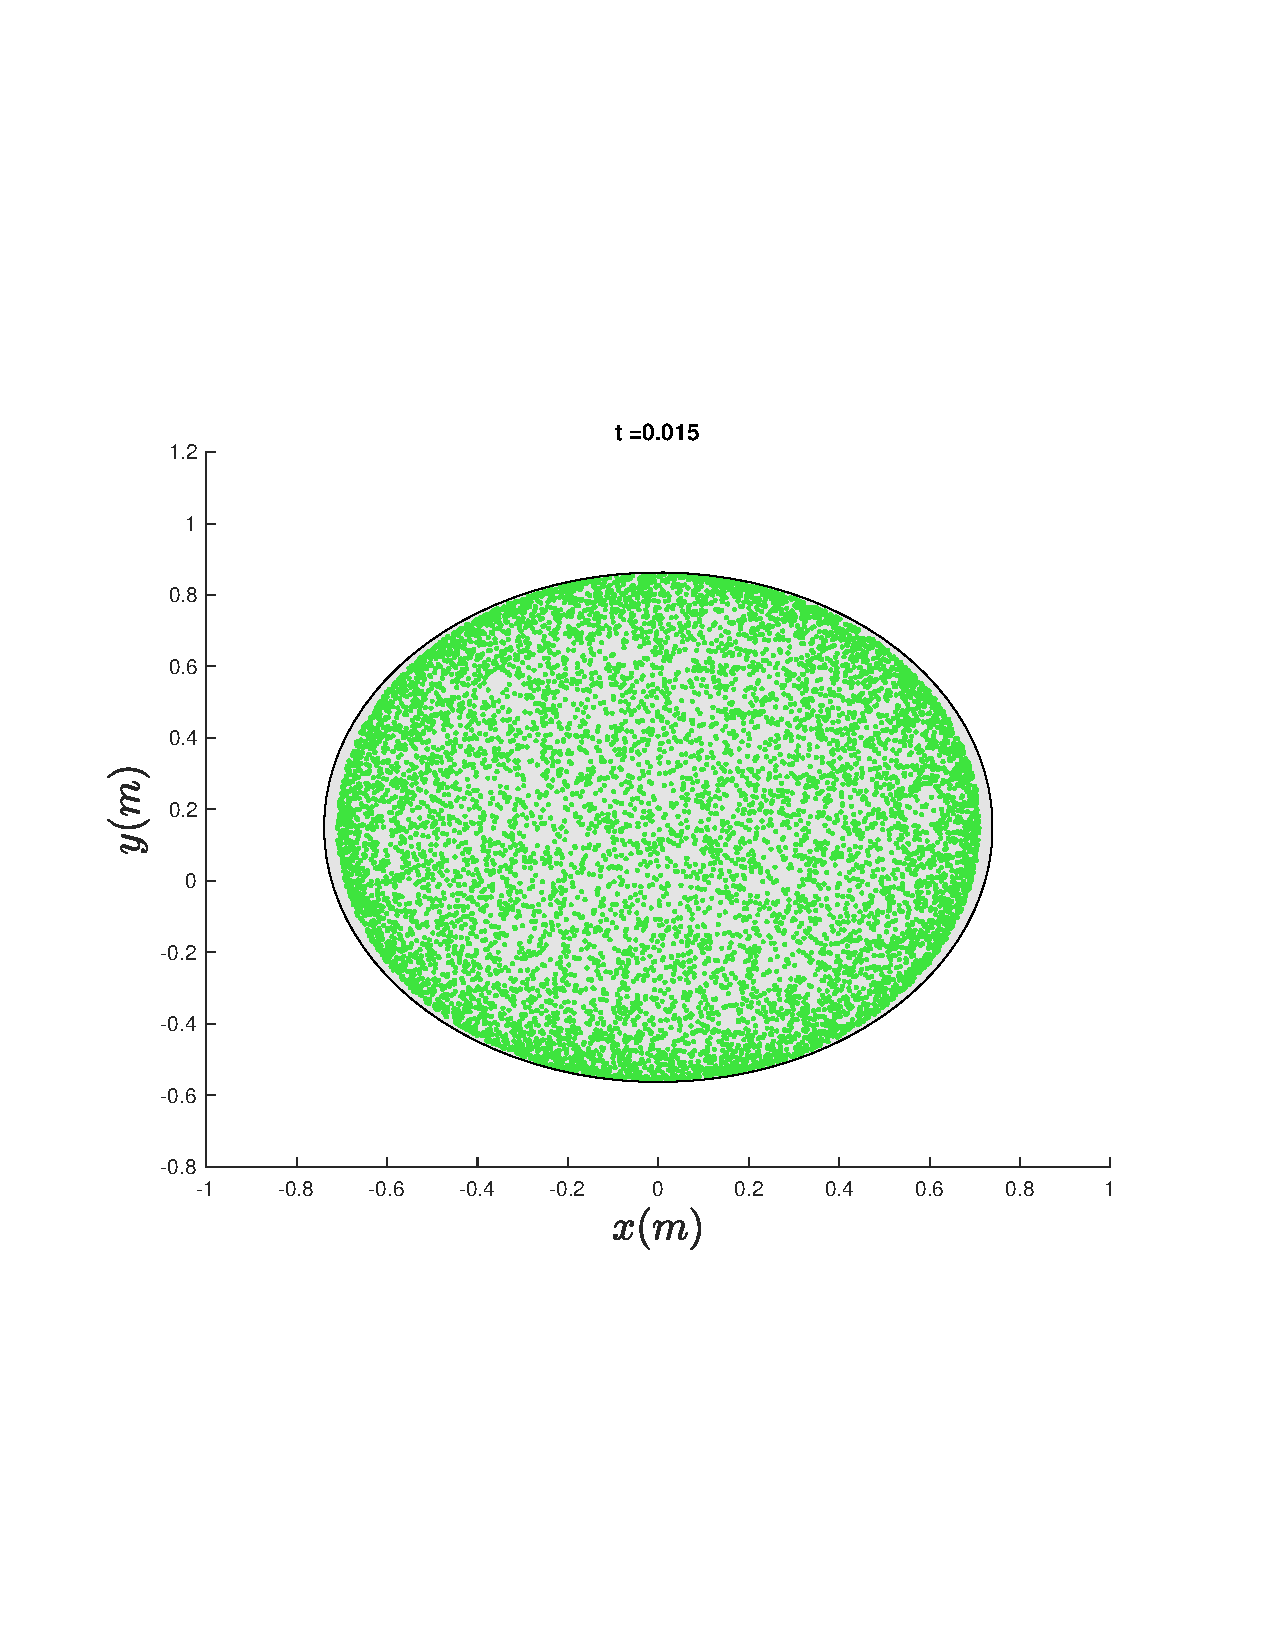
\includegraphics[width=\textwidth]{figures/method/FunnelSimOverlaid3funnel-1}
      \end{minipage}%
      % 
      \\
      % 
      \begin{minipage}[b]{0.5\textwidth}
        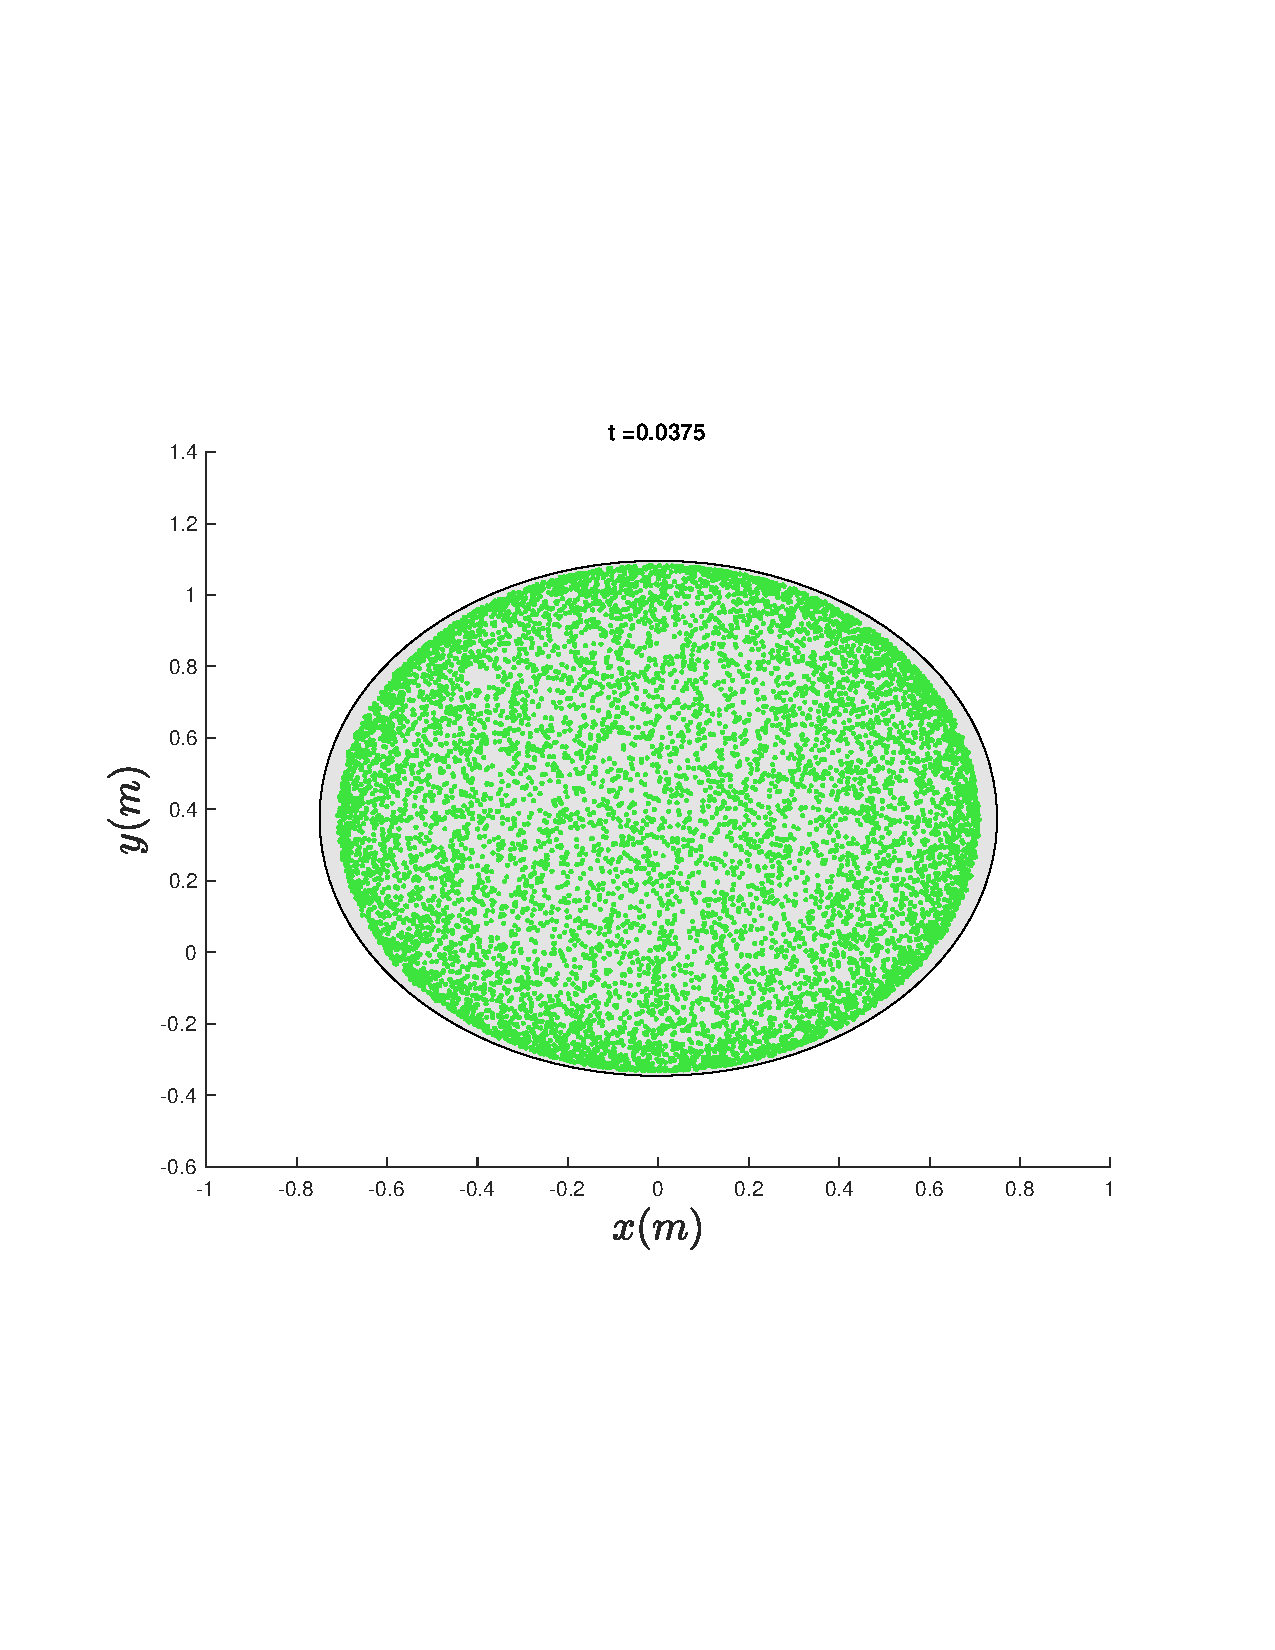
\includegraphics[width=\textwidth]{figures/method/FunnelSimOverlaid6funnel-1}
      \end{minipage}%
      % 
      \begin{minipage}[b]{0.5\textwidth}
        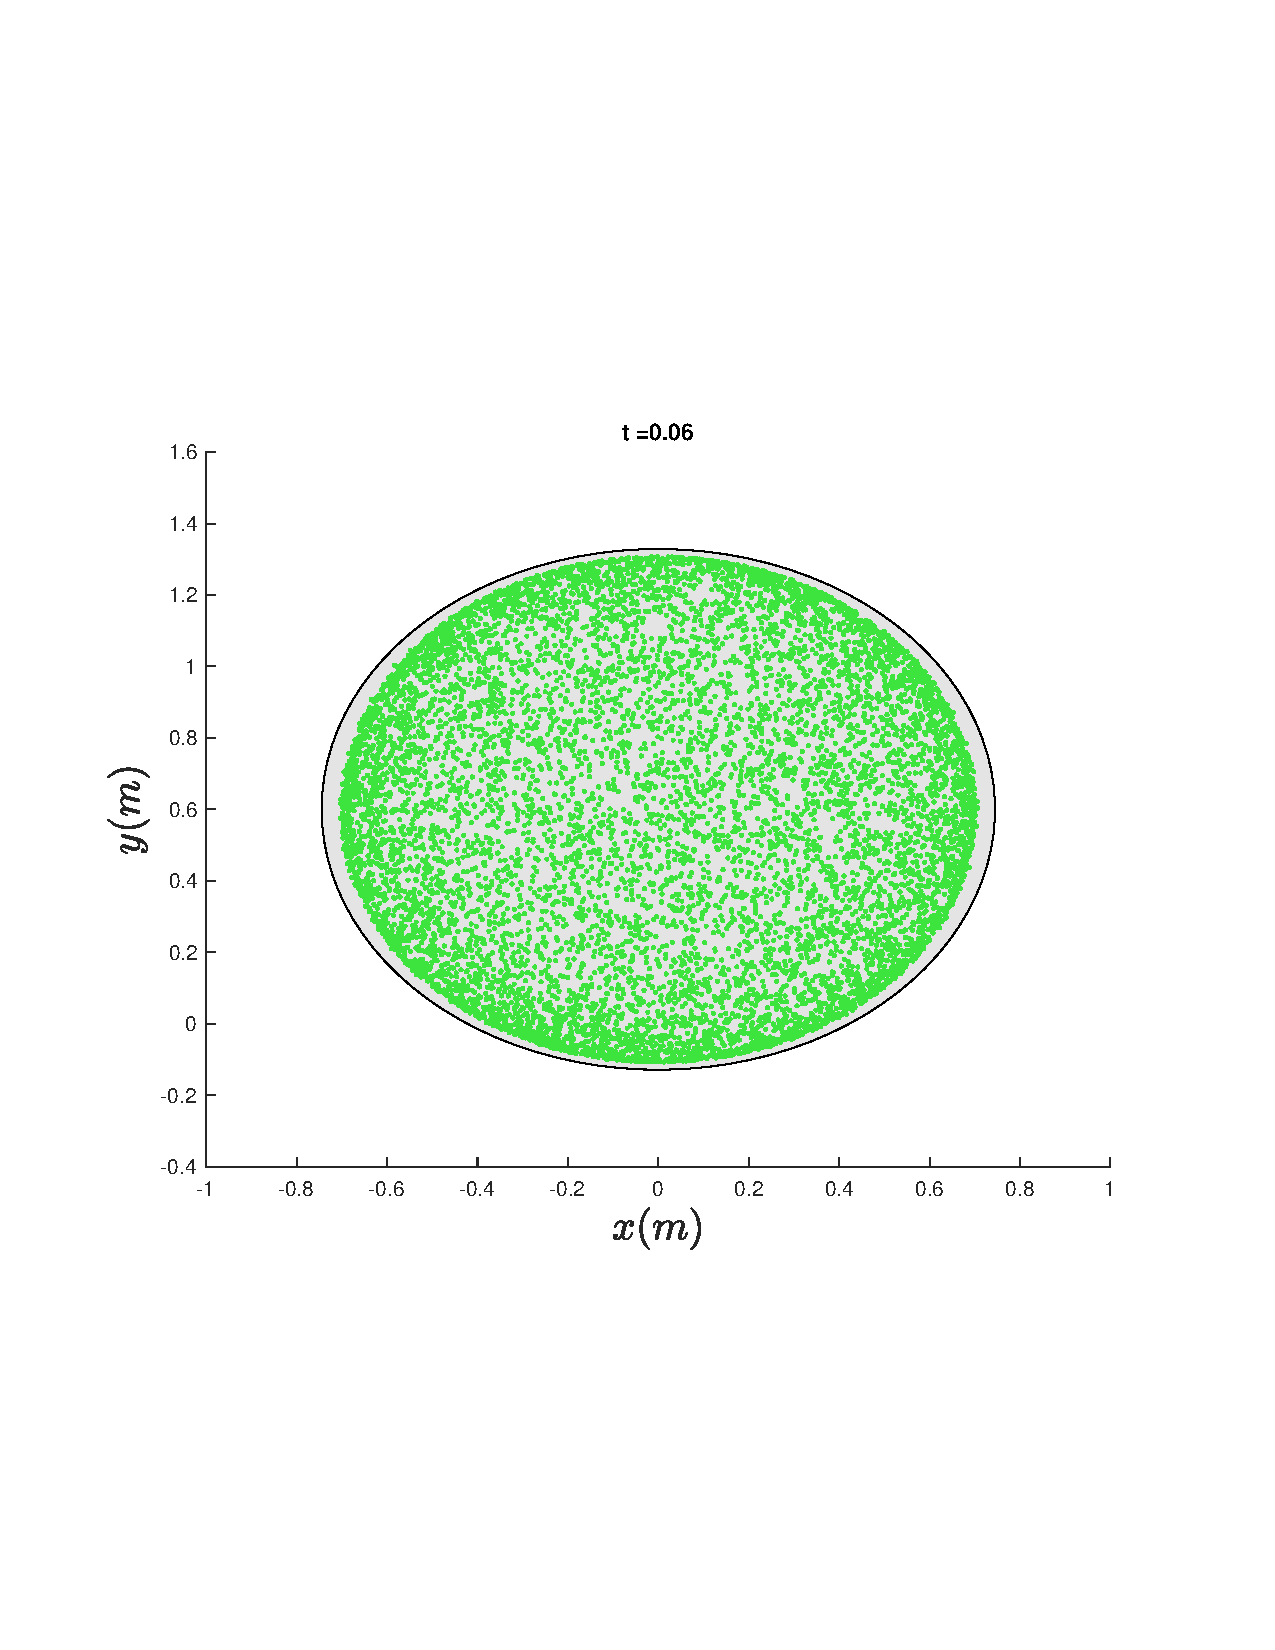
\includegraphics[width=\textwidth]{figures/method/FunnelSimOverlaid9funnel-1}
      \end{minipage}%
      % 
      \\
      % 
      \begin{minipage}[b]{0.5\textwidth}
        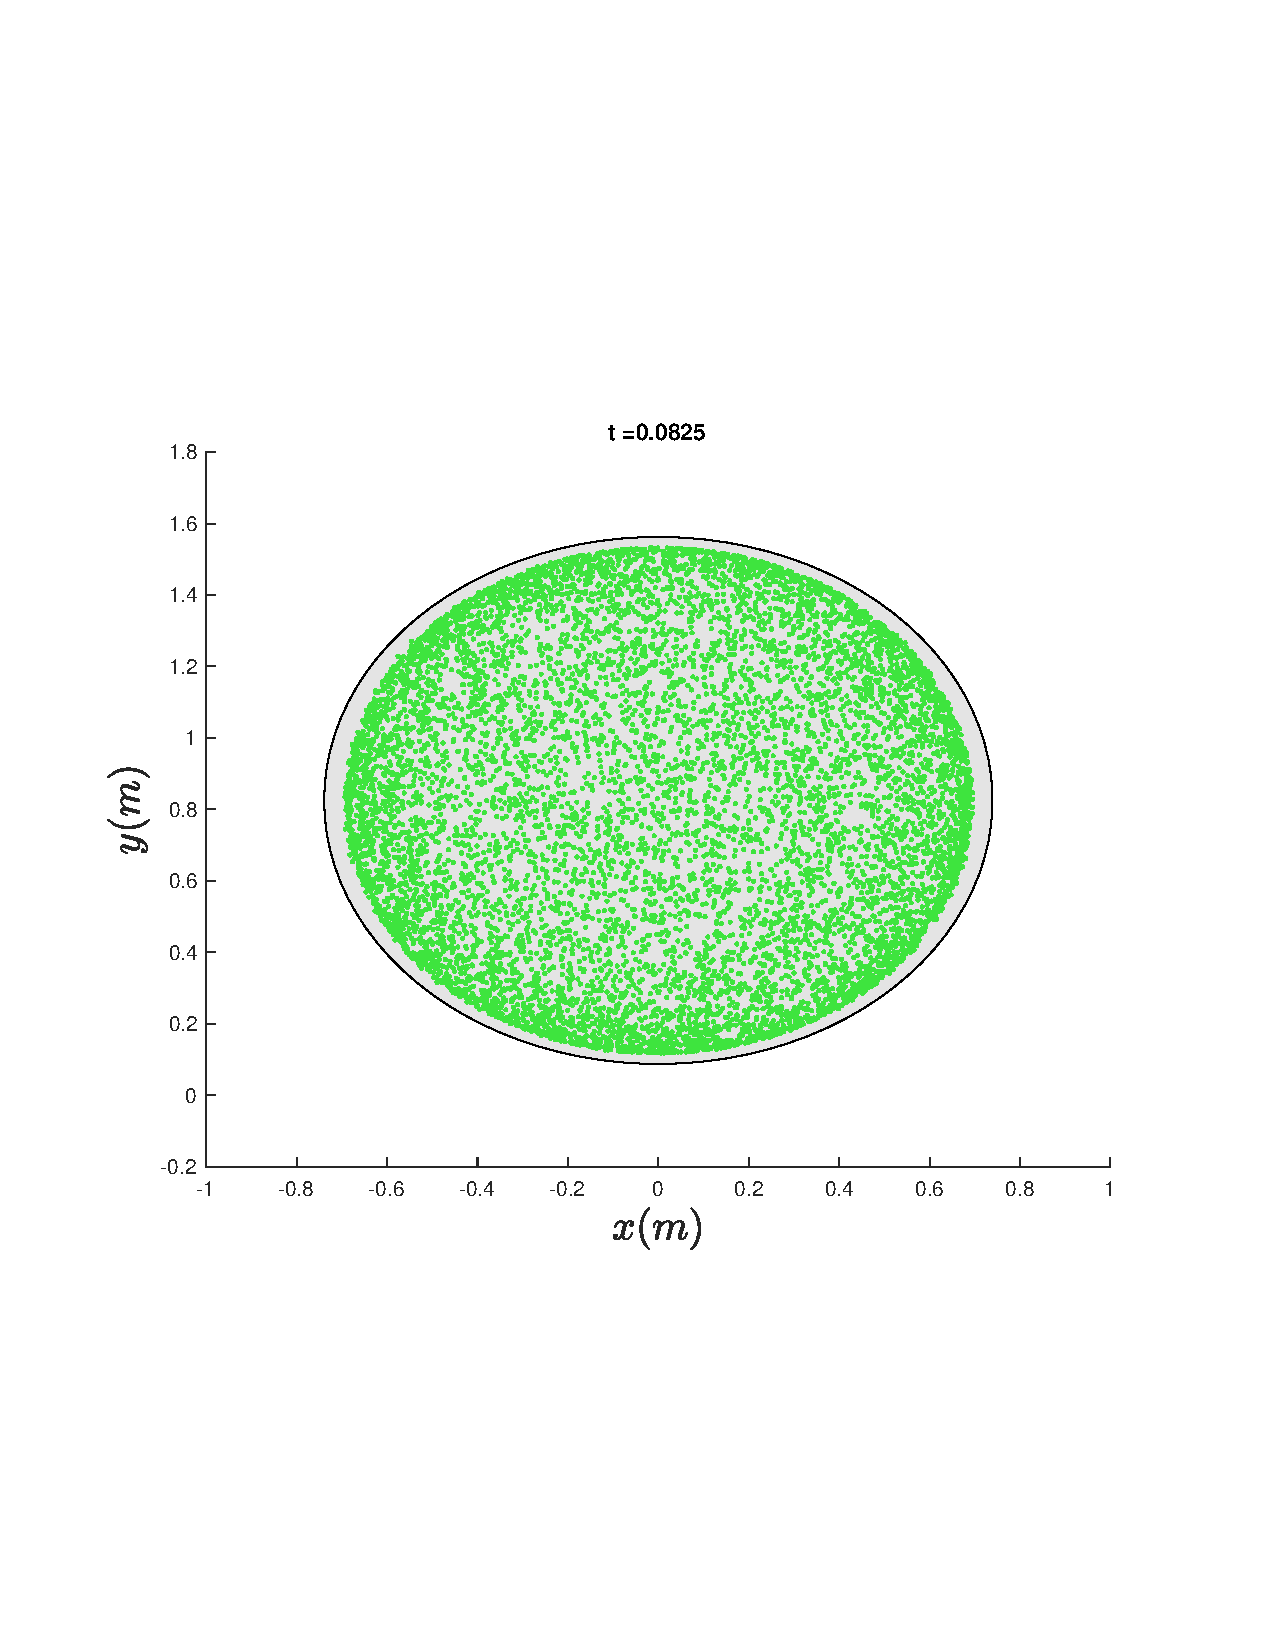
\includegraphics[width=\textwidth]{figures/method/FunnelSimOverlaid12funnel-1}
      \end{minipage}%
      % 
      \begin{minipage}[b]{0.5\textwidth}
        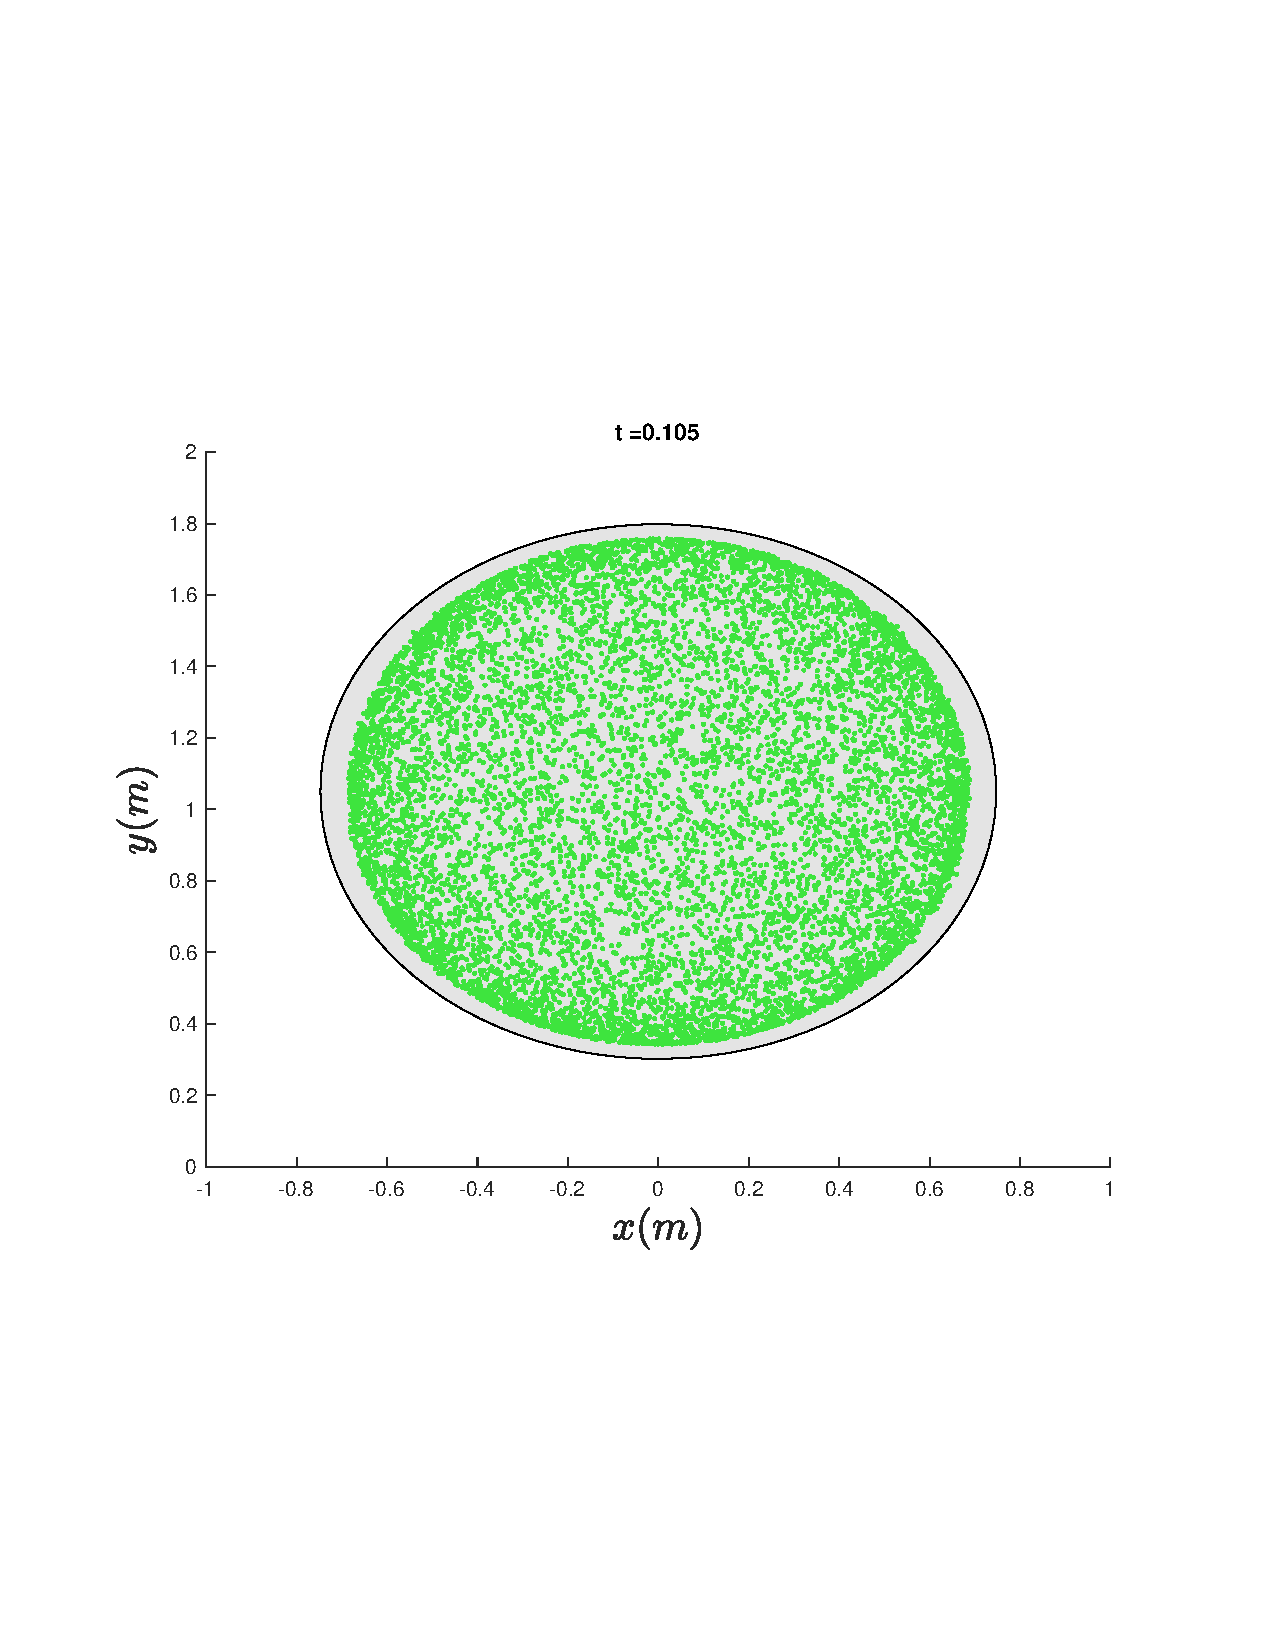
\includegraphics[width=\textwidth]{figures/method/FunnelSimOverlaid15funnel-1}
      \end{minipage}%
      % 
      \\
      % 
      \begin{minipage}[b]{0.5\textwidth}
        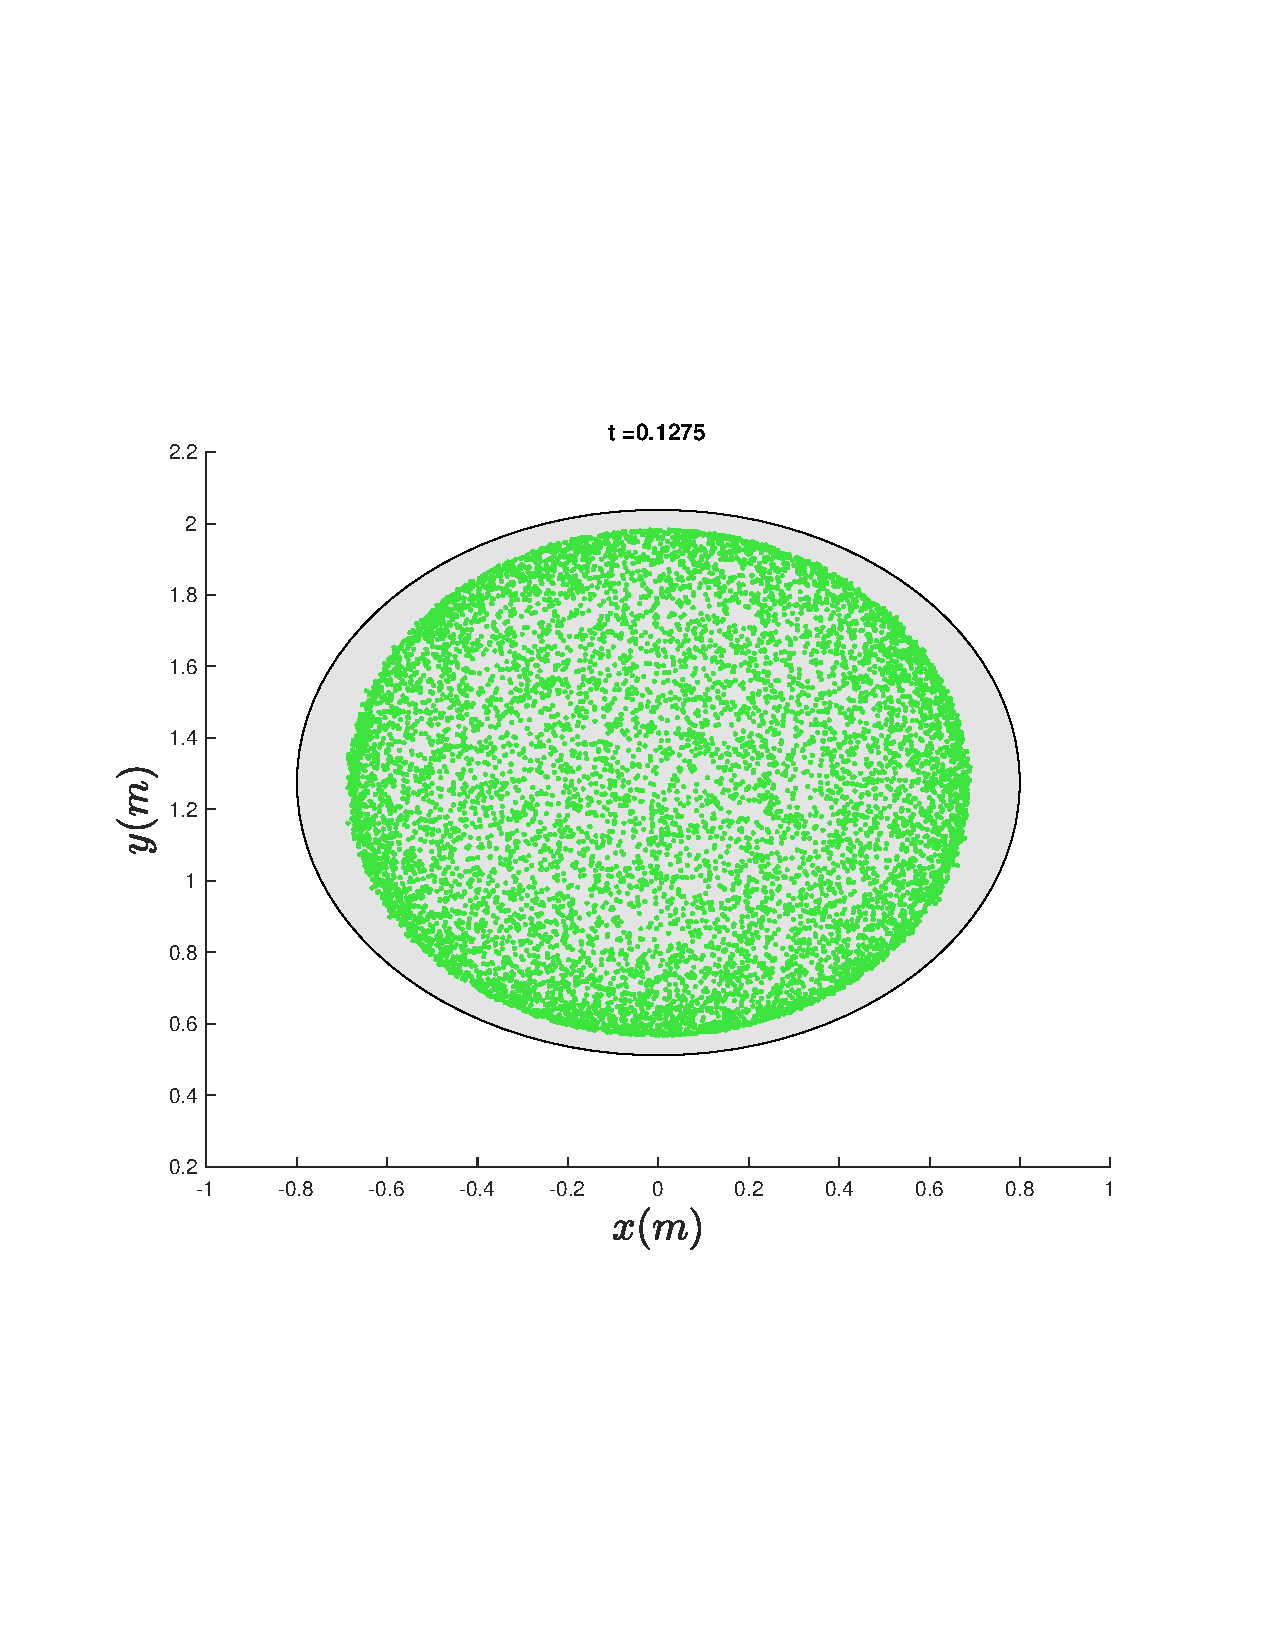
\includegraphics[width=\textwidth]{figures/method/FunnelSimOverlaid18funnel-1}
      \end{minipage}%
      % 
      \begin{minipage}[b]{0.5\textwidth}
        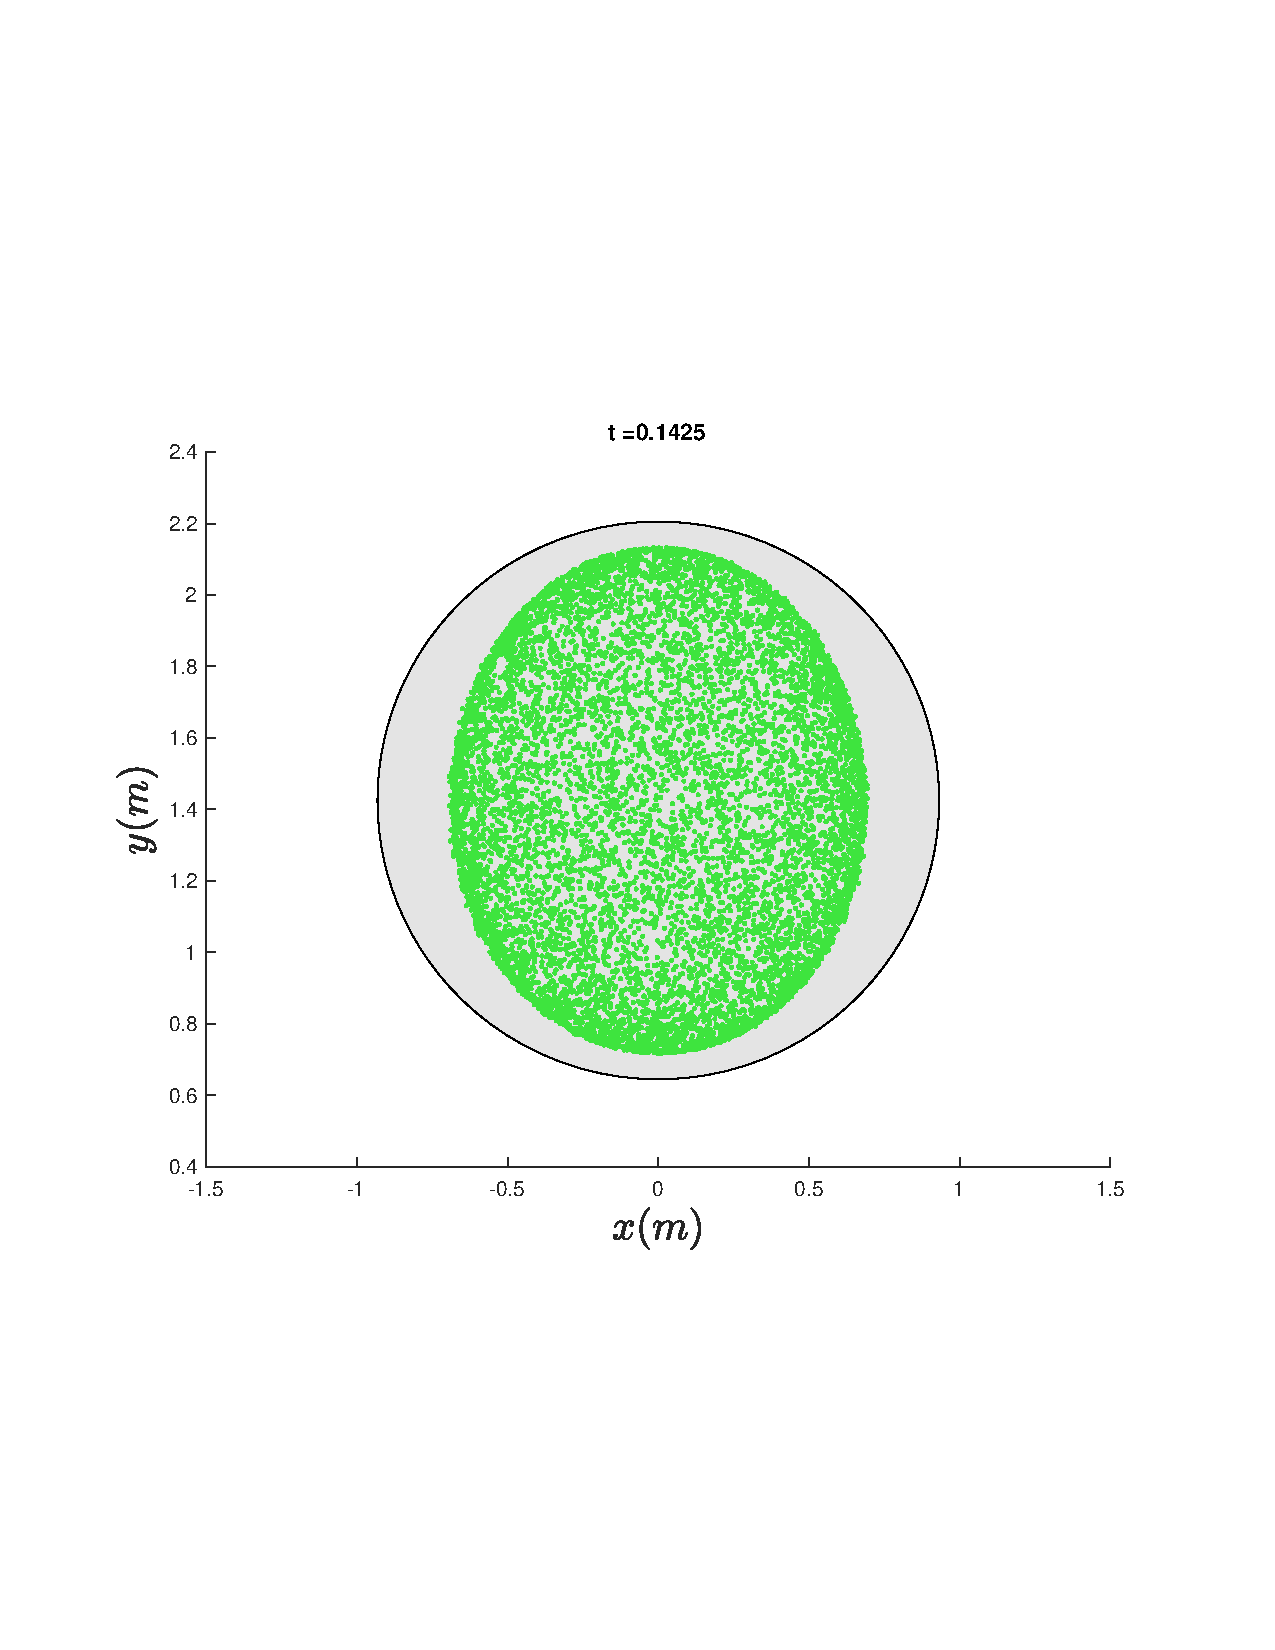
\includegraphics[width=\textwidth]{figures/method/FunnelSimOverlaid20funnel-1}
      \end{minipage}%
    \end{minipage} % End Left subfig
  }
  % 
  % \; % Left and right split
  % 
  \fbox{%
    \begin{minipage}{0.5\textwidth} % Right subfig
      % 
      \begin{minipage}[b]{0.5\textwidth} % Inner left
        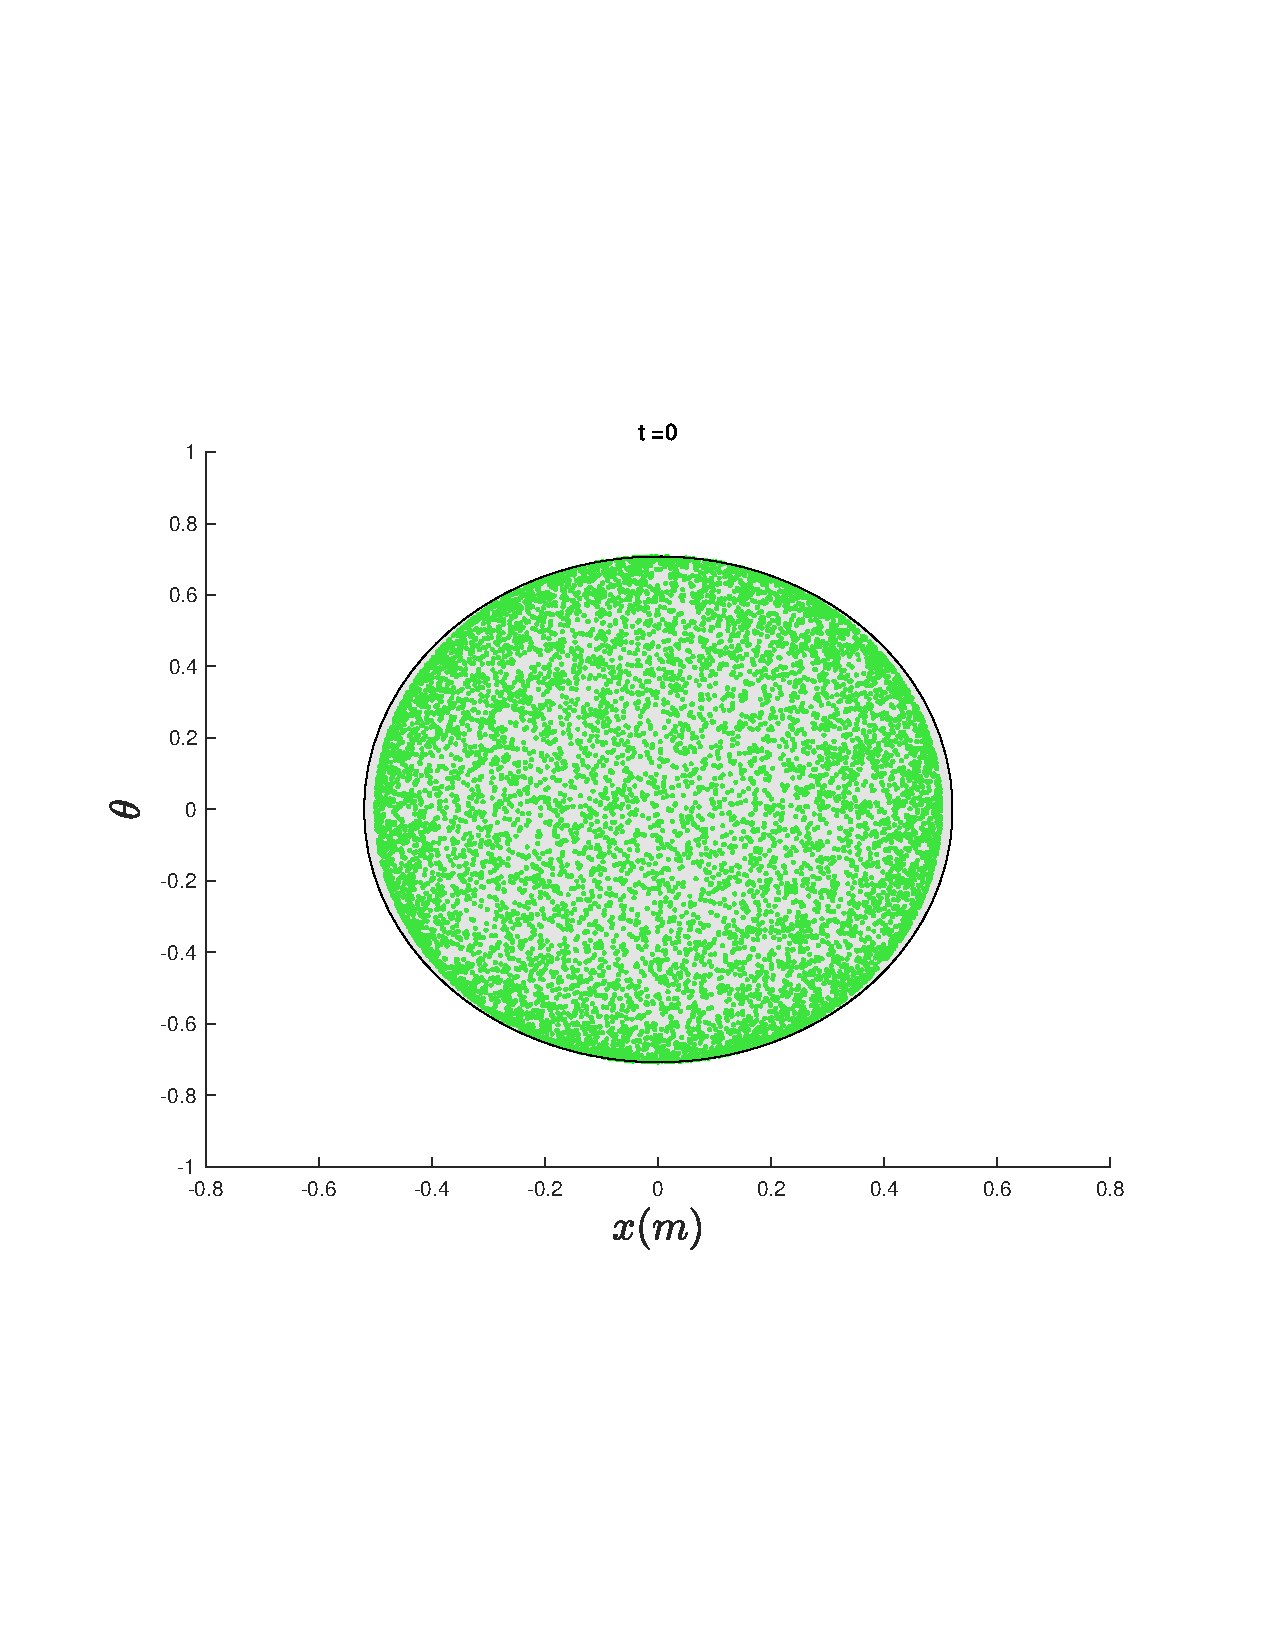
\includegraphics[width=\textwidth]{figures/method/FunnelSimOverlaid1funnel-1y-theta}
      \end{minipage}%
      % 
      \begin{minipage}[b]{0.5\textwidth}
        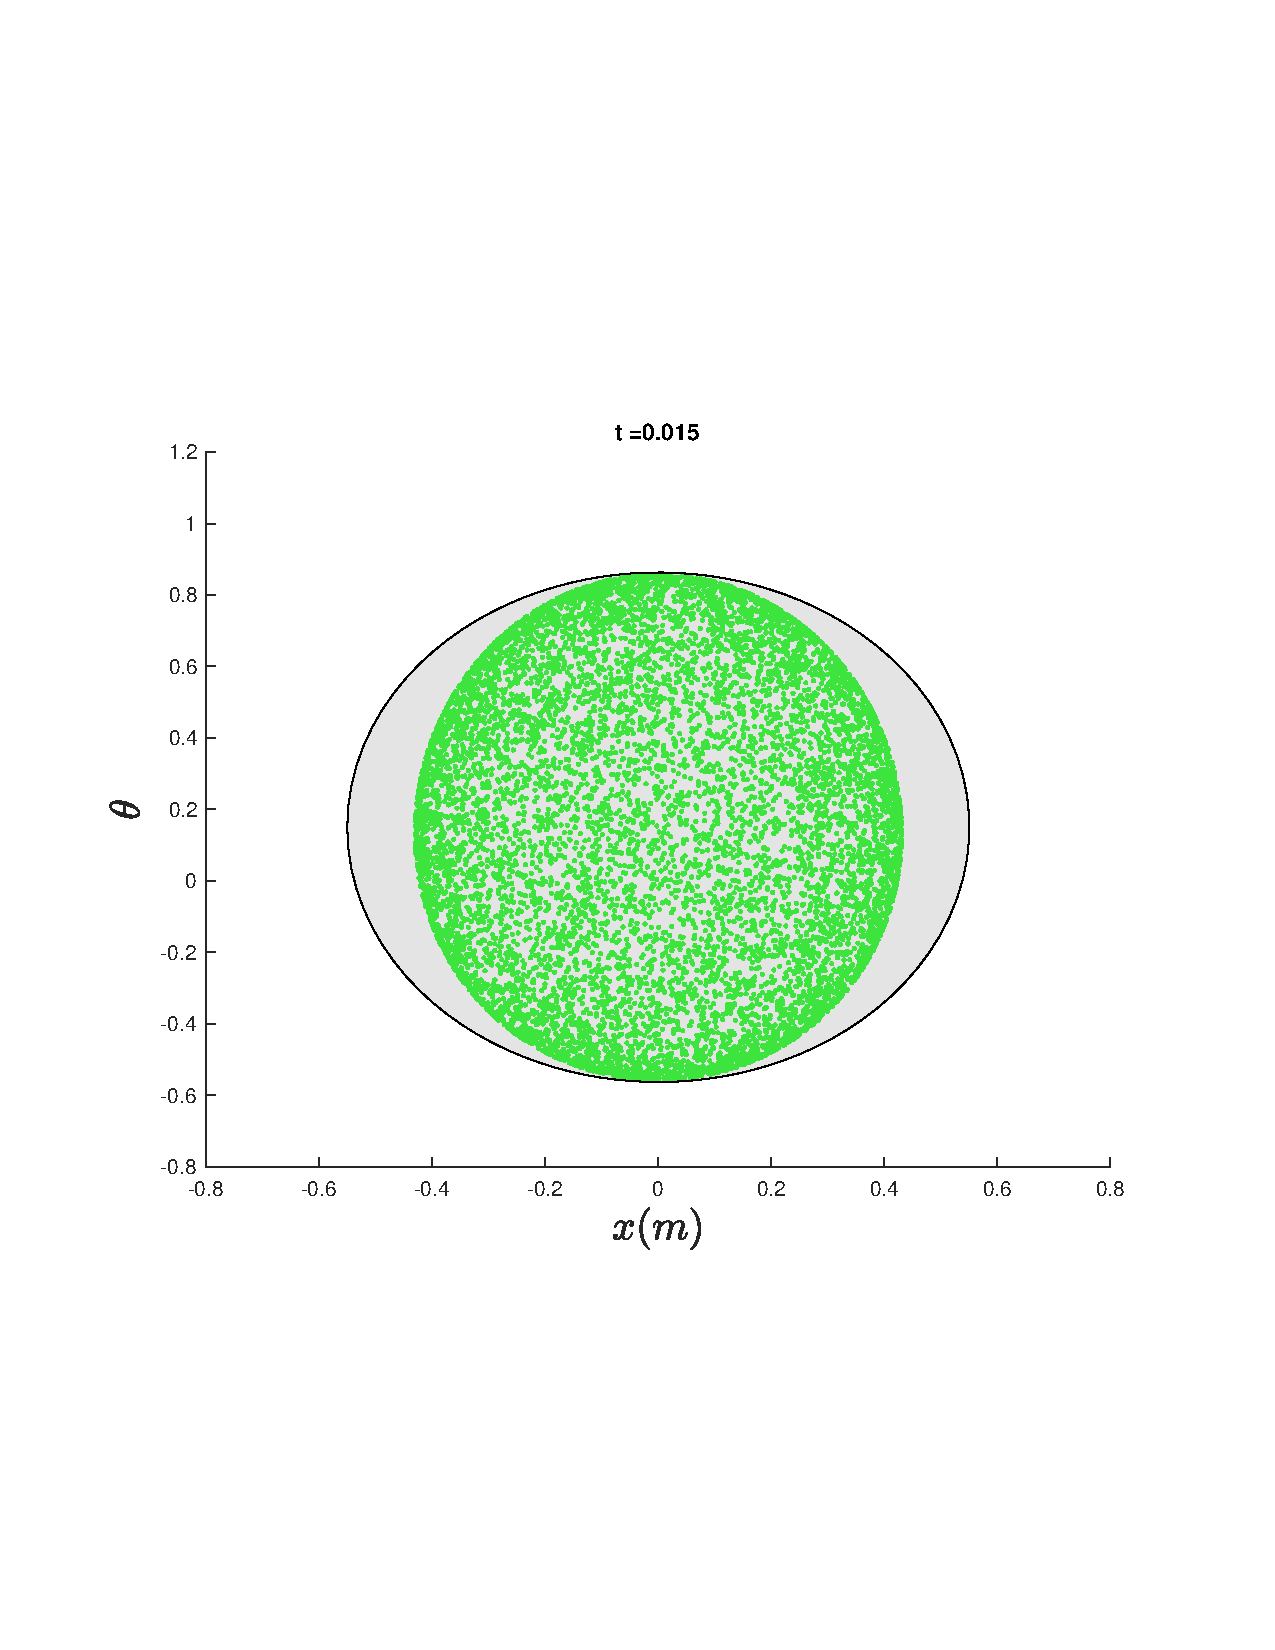
\includegraphics[width=\textwidth]{figures/method/FunnelSimOverlaid3funnel-1y-theta}
      \end{minipage}%
      % 
      \\
      % 
      \begin{minipage}[b]{0.5\textwidth}
        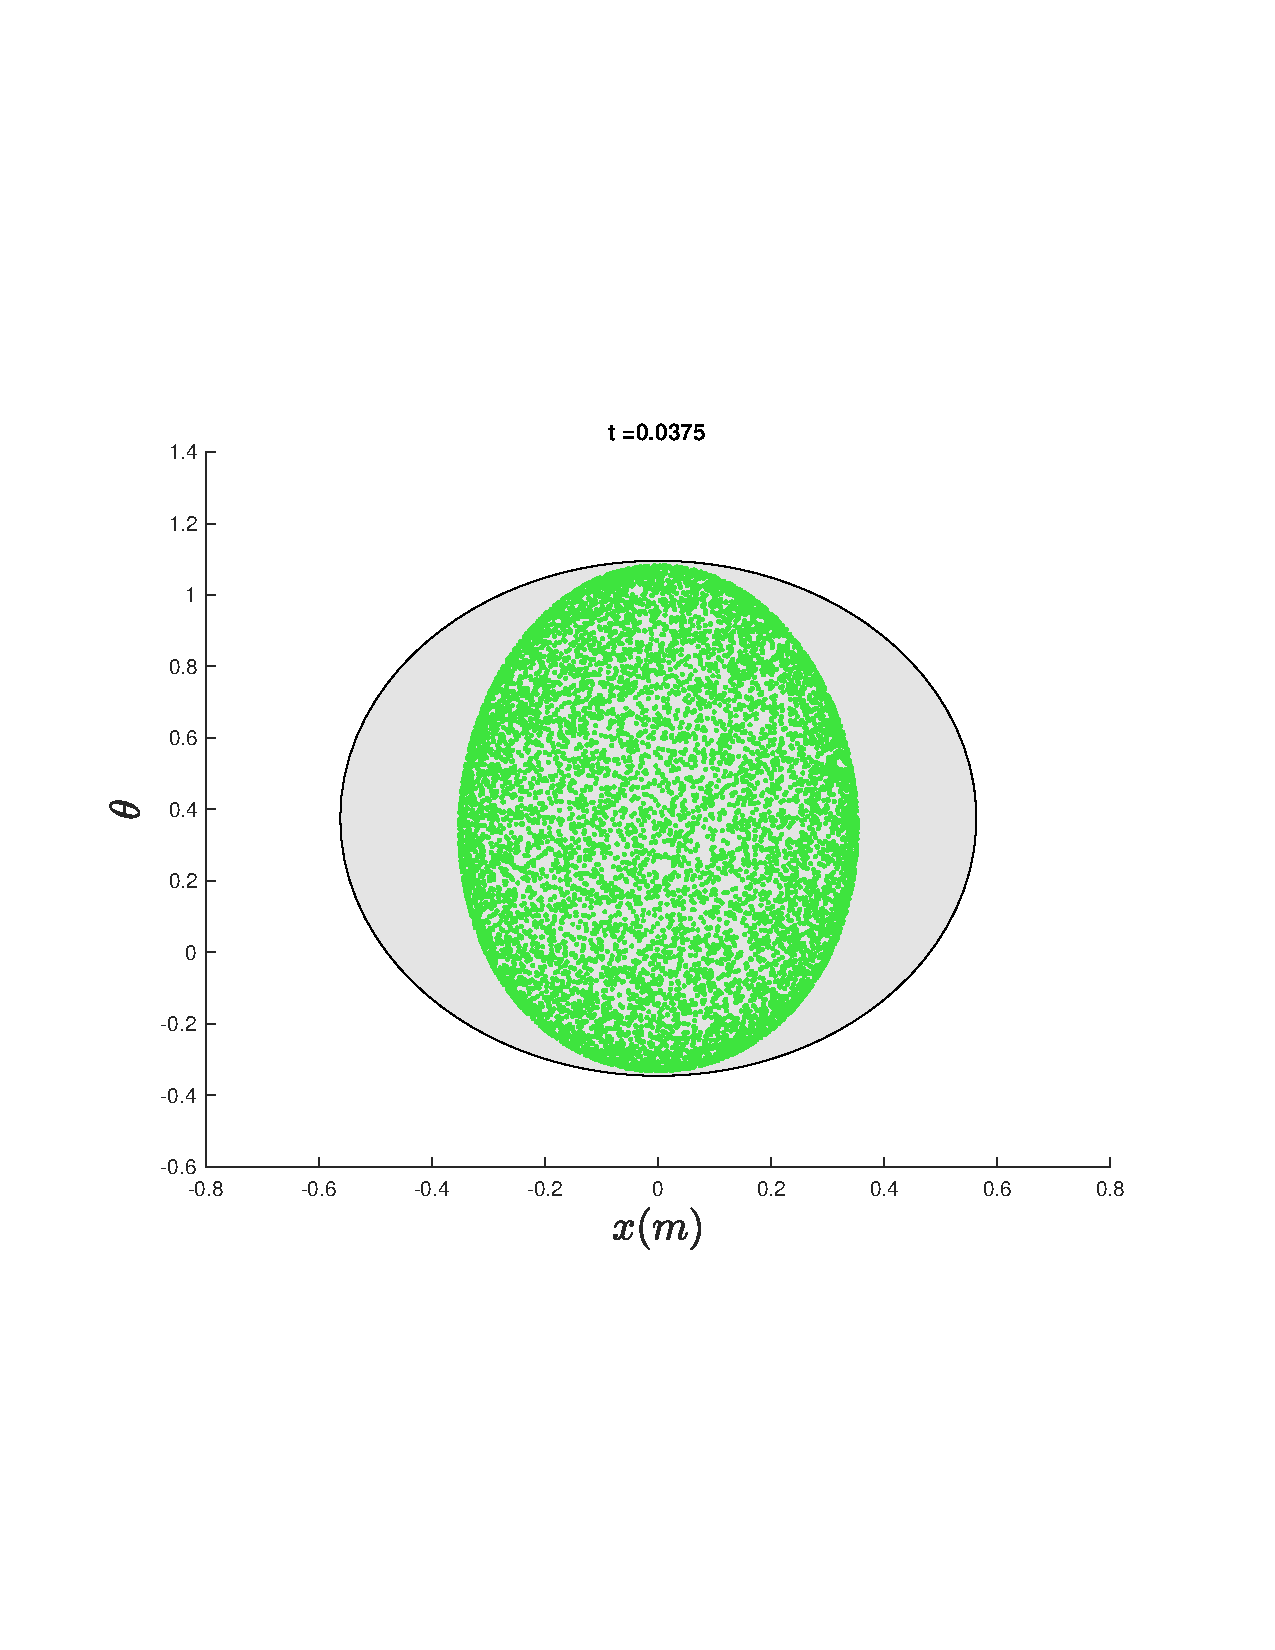
\includegraphics[width=\textwidth]{figures/method/FunnelSimOverlaid6funnel-1y-theta}
      \end{minipage}%
      % 
      \begin{minipage}[b]{0.5\textwidth}
        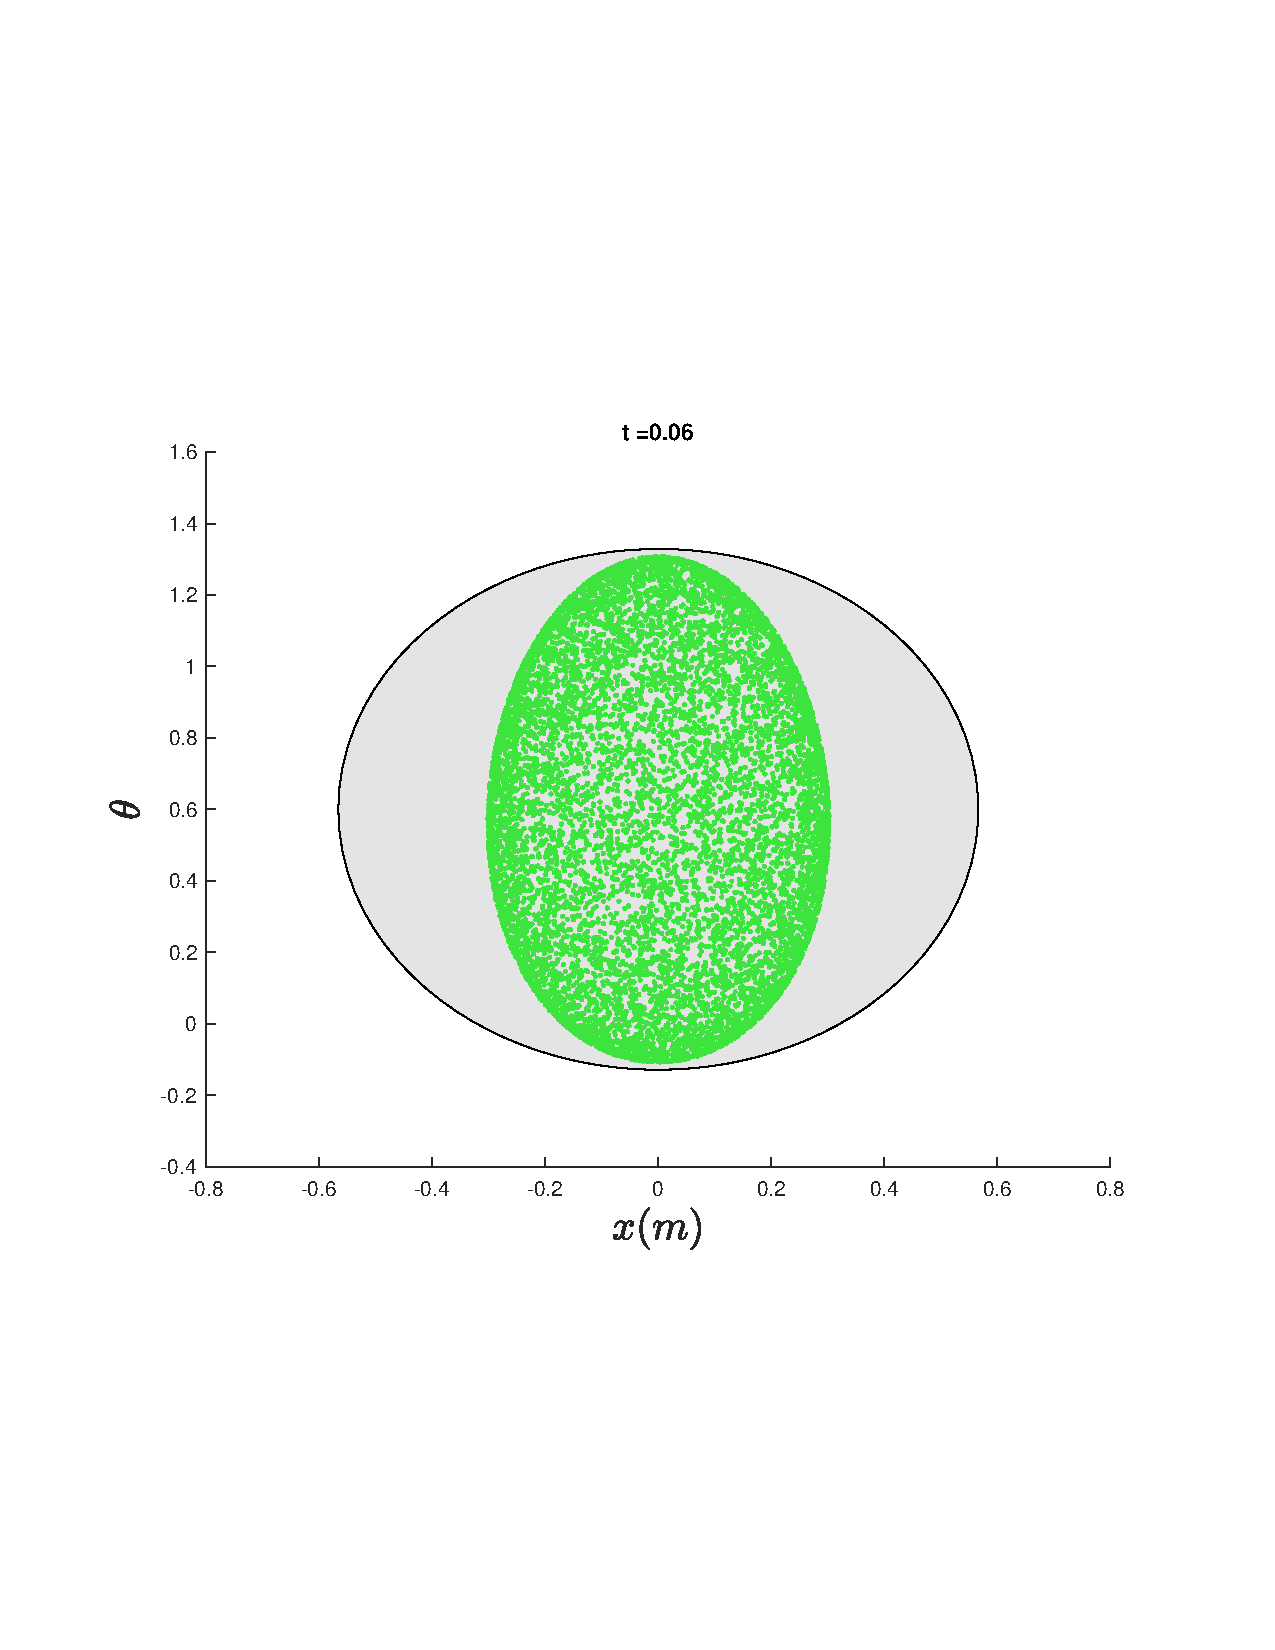
\includegraphics[width=\textwidth]{figures/method/FunnelSimOverlaid9funnel-1y-theta}
      \end{minipage}%
      % 
      \\
      % 
      \begin{minipage}[b]{0.5\textwidth}
        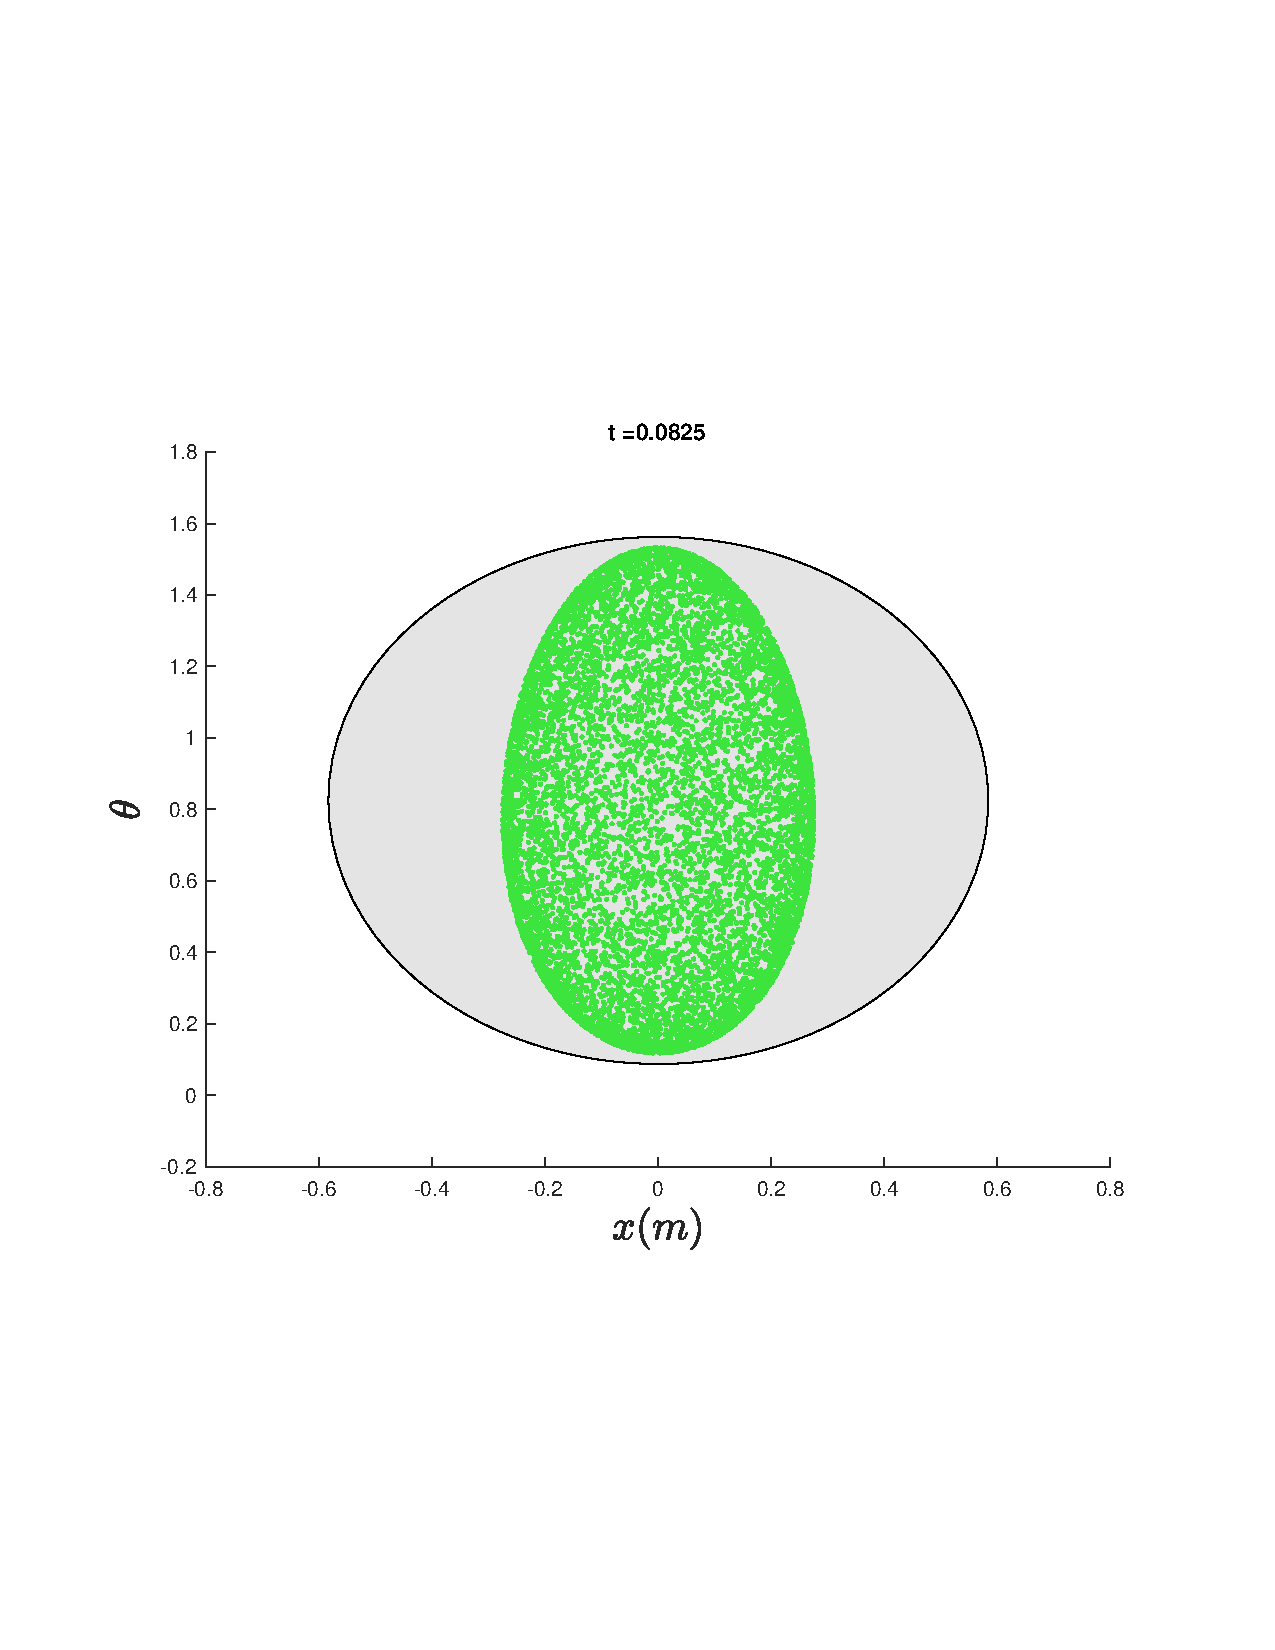
\includegraphics[width=\textwidth]{figures/method/FunnelSimOverlaid12funnel-1y-theta}
      \end{minipage}%
      % 
      \begin{minipage}[b]{0.5\textwidth}
        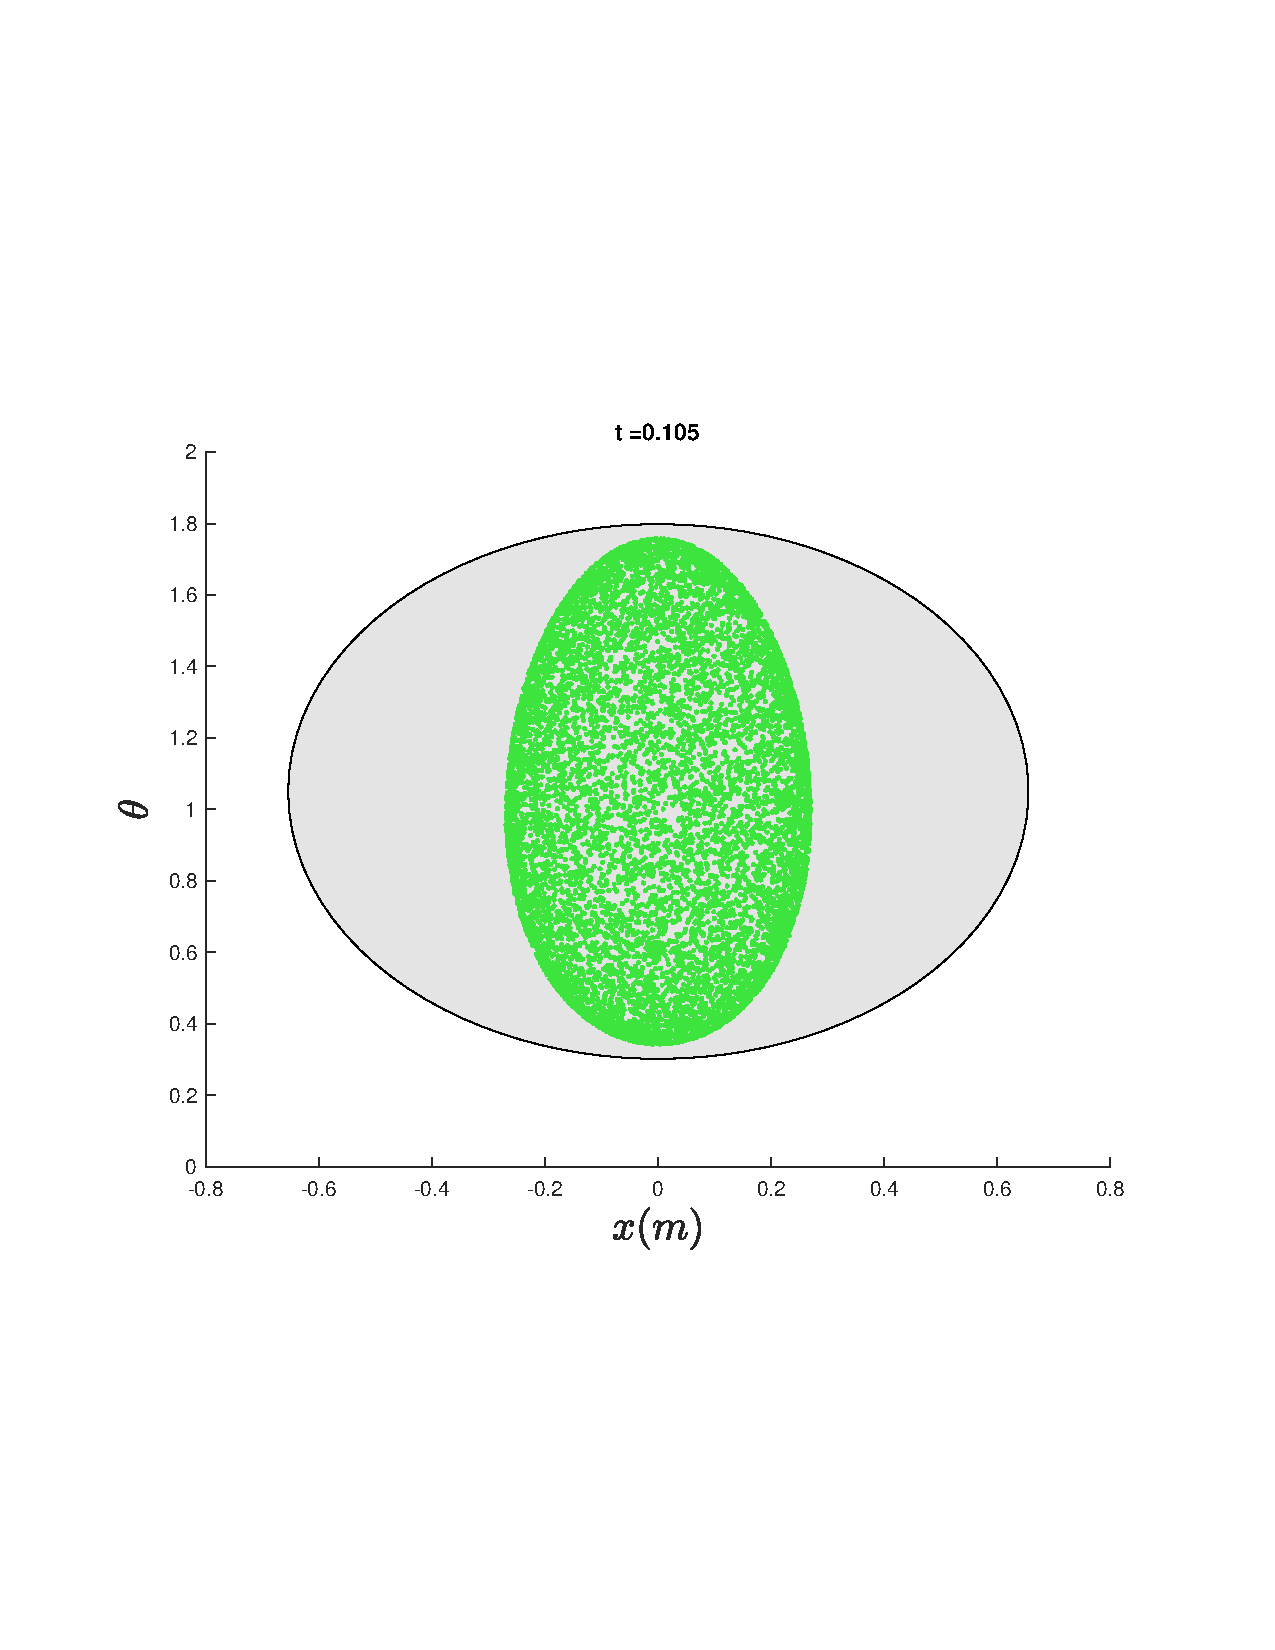
\includegraphics[width=\textwidth]{figures/method/FunnelSimOverlaid15funnel-1y-theta}
      \end{minipage}%
      % 
      \\
      % 
      \begin{minipage}[b]{0.5\textwidth}
        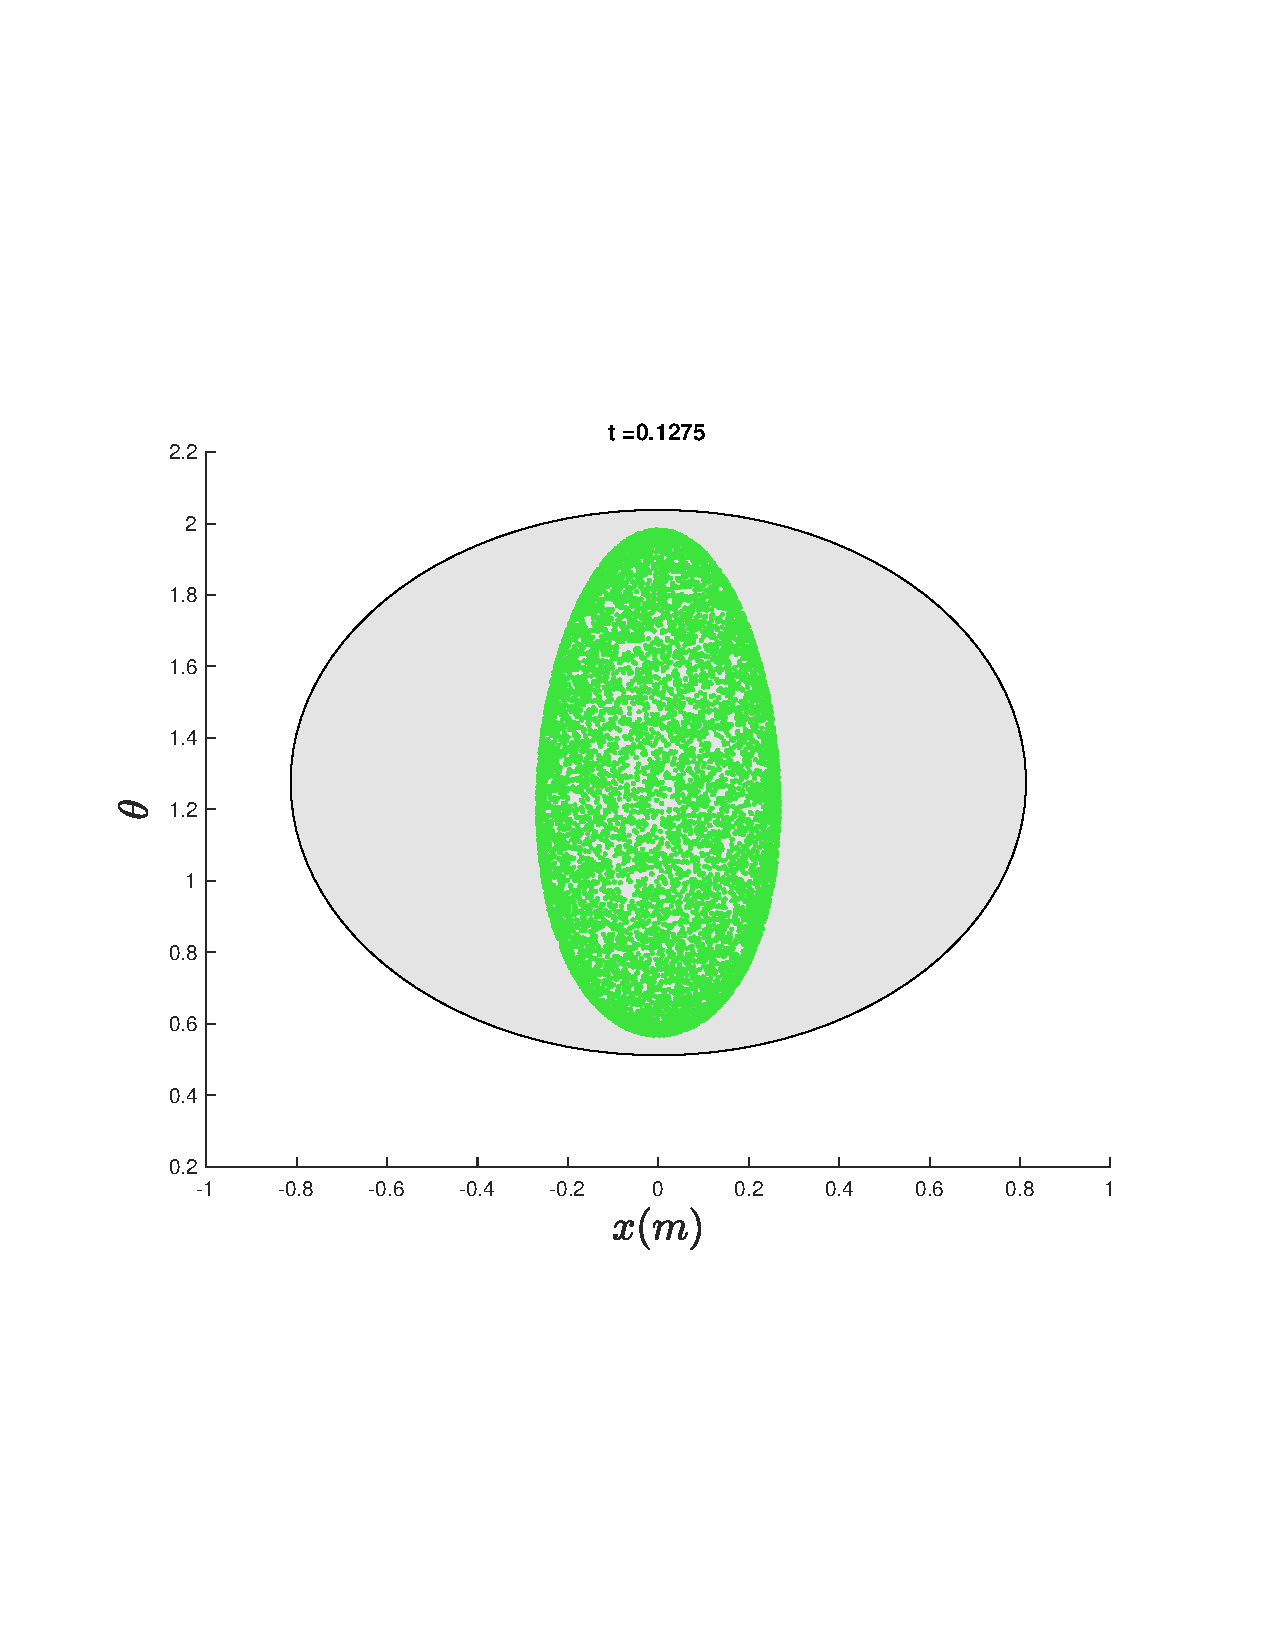
\includegraphics[width=\textwidth]{figures/method/FunnelSimOverlaid18funnel-1y-theta}
      \end{minipage}%
      % 
      \begin{minipage}[b]{0.5\textwidth}
        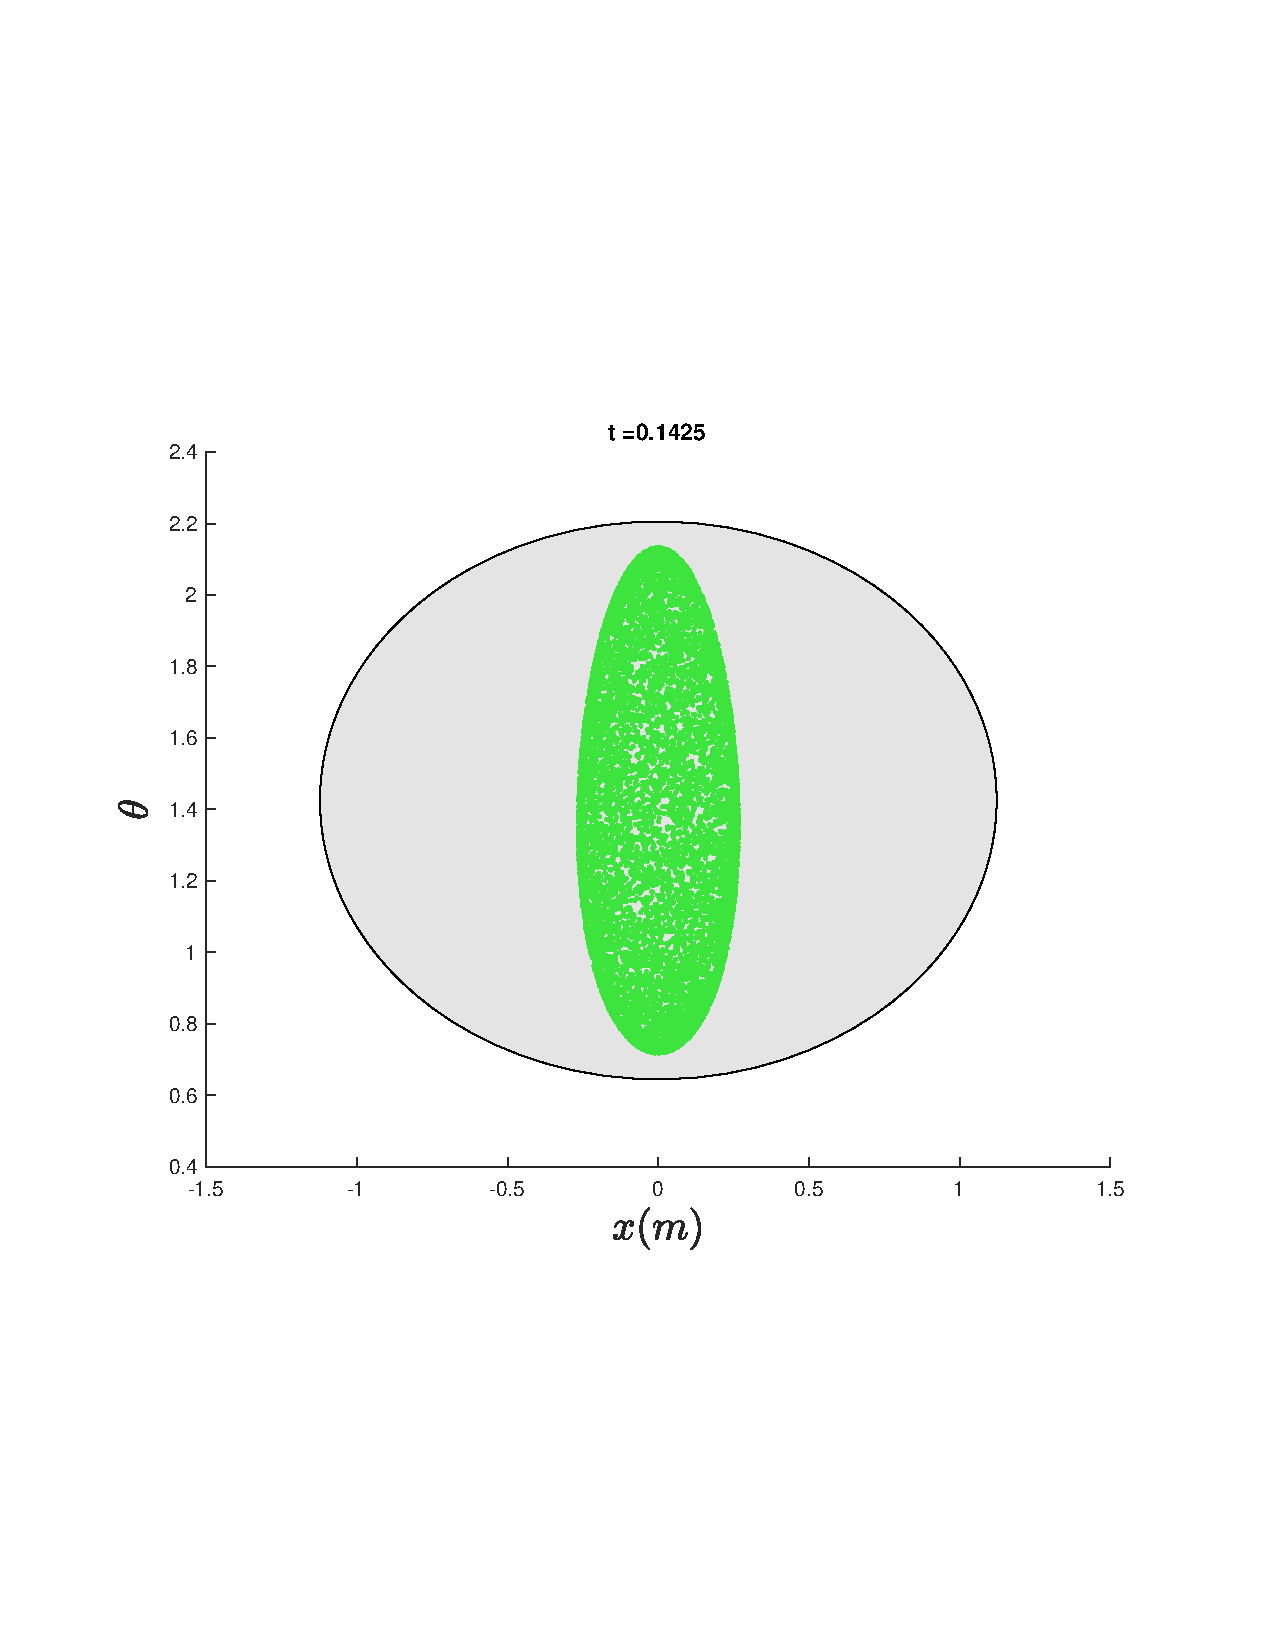
\includegraphics[width=\textwidth]{figures/method/FunnelSimOverlaid20funnel-1y-theta}
      \end{minipage}%
    \end{minipage}%
  }
\end{figure}

\subsection{The initial condition set for each funnel}

In order to stack funnels one after the other it is necessary for the funnels to
have a big inlet, and a smaller outlet as defined in hyperspace. It is from the
formulations in (ref preliminaries) to constrain the initial condition set for
each funnel. This is done with

The initial theta is limited to: (Make pretty figure with the initial conditions
for theta at each point (x,y))

\section{RRT}

With the basic framework for dealing with funnels as motion primitives
constructed, it is time to build the \ac{RRT} part of the \rrtfunnel{}
algorithm. The reason for choosing to base the global path planning framework on
the \ac{RRT} motion planning algorithm are as follows. One, it has the ability
to quickly expand deep into the search-space, and then later progress towards a
finer sampling, which is valuable as it avoids local minima. Two, the \ac{RRT}
algorithm is easily extensible to larger state spaces, and thus adding to the
generality of the \rrtfunnel{} algorithm, such that it can be adapted to fit a
wide range of dynamical systems, as well that it has only three main components
that needs to be in place in order for successful path planning to happen in an
arbitrary configuration space. This is beneficial as most of the complexity
accompanied with the planning problem (like uncertainty and controller
calculations) has already been handled by the \ac{SOS} framework, and hence the
\ac{RRT} algorithm need only concern itself with stacking one robust motion
primitive after the other without any concern for the complexities mentioned
above.

\subsection{Uniform sampling in SE(2)}

As mentioned in section~\nameref{sec:rrt-algorithm-intro}, the \ac{RRT}
algorithm needs uniform sampling of the state space in order for it to function
optimally, as over- or under-sampling certain parts of the state space can lead
to poor performance. Therefore one needs to be careful when sampling from a
configuration space with non Euclidean
topology~\cite{kuffnerEffectiveSamplingDistance2004}.

If sampling from a configuration space which are formed strictly from Cartesian
products of the form \(X = X_1\times X_2\times \cdots \times X_n\), and each
Cartesian space is sampled uniformly, then the product will also be uniformly
sampled. One needs to be more careful when dealing with rotations however, as
the probability density measure can become non-uniform~\cite{Lav06}. Take the
polar coordinates as an example. Sampling uniformly from \(r\) and \(\theta\)
does not form a uniform sample product, as the \(pdf\) function will have a
higher probability density near the origin, as the outer circles will contain a
bigger area. For the model of a simple unicycle which moves in \(x,y,\theta\)
the samples can be generated from
From~\cite{kuffnerEffectiveSamplingDistance2004} the samples can be generated
uniformly on the topological cylinder through
\[
  (x,y,\theta) = (\mathnormal{X}_{dim}rand, \mathnormal{Y}_{dim}rand,
  \mathnormal{\Theta}_{dim}rand)
\]
where \(rand\) is a random variable in the interval \([0,1)\), since for
\(SO(2)\), the rotations parameterized on \([0,1]\setminus\sim\) (where
\(\setminus\sim\) means that 0 and 1 are identified) can be multiplied by a
fixed constant, such as for \(2\pi\) which means that sampling will be uniform
in the configuration space of the robot from a simple Cartesian product of
uniform random variables~\cite{Lav06}.

\subsection{Distance in configuration space}

Introducing a function which Measures distance between two points in
configuration space introduces a metric space on the underlying configuration
space \((\modelconfigurationspace{},\rho)\), where \(\rho\) is a distance
function. Finding a good distance function for the metric space at hand is a
hard problem. In general the ideal metric would have been the actual
\textit{cost-to-go} function for the system at hand. However calculating the
actual cost-to-go is equivalent to solving the original motion planning problem,
and is hence not viable~\cite{pengchengReducingMetricSensitivity2001}.

So, in order for the \rrtfunnel{} algorithm to efficiently explore the state
space it must have a good measure of distance between different poses in space,
without actually solving the planning problem anew. For a problem in the
Cartesian plane it is common to use the Euclidean distance, however, this is not
a good distance metric for non-holonomic vehicles, as it does not incorporate
the possible constraints of the system function, and has little bearing on the
actual cost-to-go of the system~\cite{parkFeedbackMotionPlanning2015}. In fact,
for sampling based planners such as the \ac{RRT}, the configuration space is
only sufficiently explored in the case where the distance function reflects the
true cost-to-go function~\cite{pengchengReducingMetricSensitivity2001}. Hence,
all other metrics will be a compromise of complexity and time vs efficiency.

Normally the \ac{RRT} algorithm splits the extension part into two sections. One
for identifying the closest node in the tree, and second one for the closest
extension that can be added onto the tree itself. Here a different distance
metric can be employed in each step. To reflect on the difficulty of creating a
general distance metric function have a look at the unicycle model
from~\cref{eq:model-dynamics}. From inspection it is seen that the model is not
able to instantaneously move in a direction orthogonal to the direction of
travel, as is seen in~\cref{fig:non-holonomic-vehicle-euclidean-weakness}. Here
the distance between two points might be small in the sense of a regular
Euclidean distance metric, but due to the differential constraints on the system
model, the vehicle actually has to move far in order to reach the sought
configuration.

The \rrtfunnel{} algorithm will use the same metric for both the closest node
and in the extend operation on the funnel graph. The metric chosen is a modified
Euclidean metric which weights the angle \((\theta)\) depending on how close the
vehicle is to the final configuration and is defined as
\[
  \rho(x_{1},x_{2}) = w_{1}\norm{\mathnormal{X_{1}} - \mathnormal{X_{2}}} +
  w_{2}f(\theta_1,\theta_2)
\]
and taken from~\cite{kuffnerEffectiveSamplingDistance2004}, where
\(\norm{\mathnormal{X_{1}} - \mathnormal{X_{2}}}\) is the standard Euclidean
metric, and \(f\) is a function, giving the distance between headings, and the
rotations and distance is scaled relative to the translation distance.

\begin{figure}
  \centering
  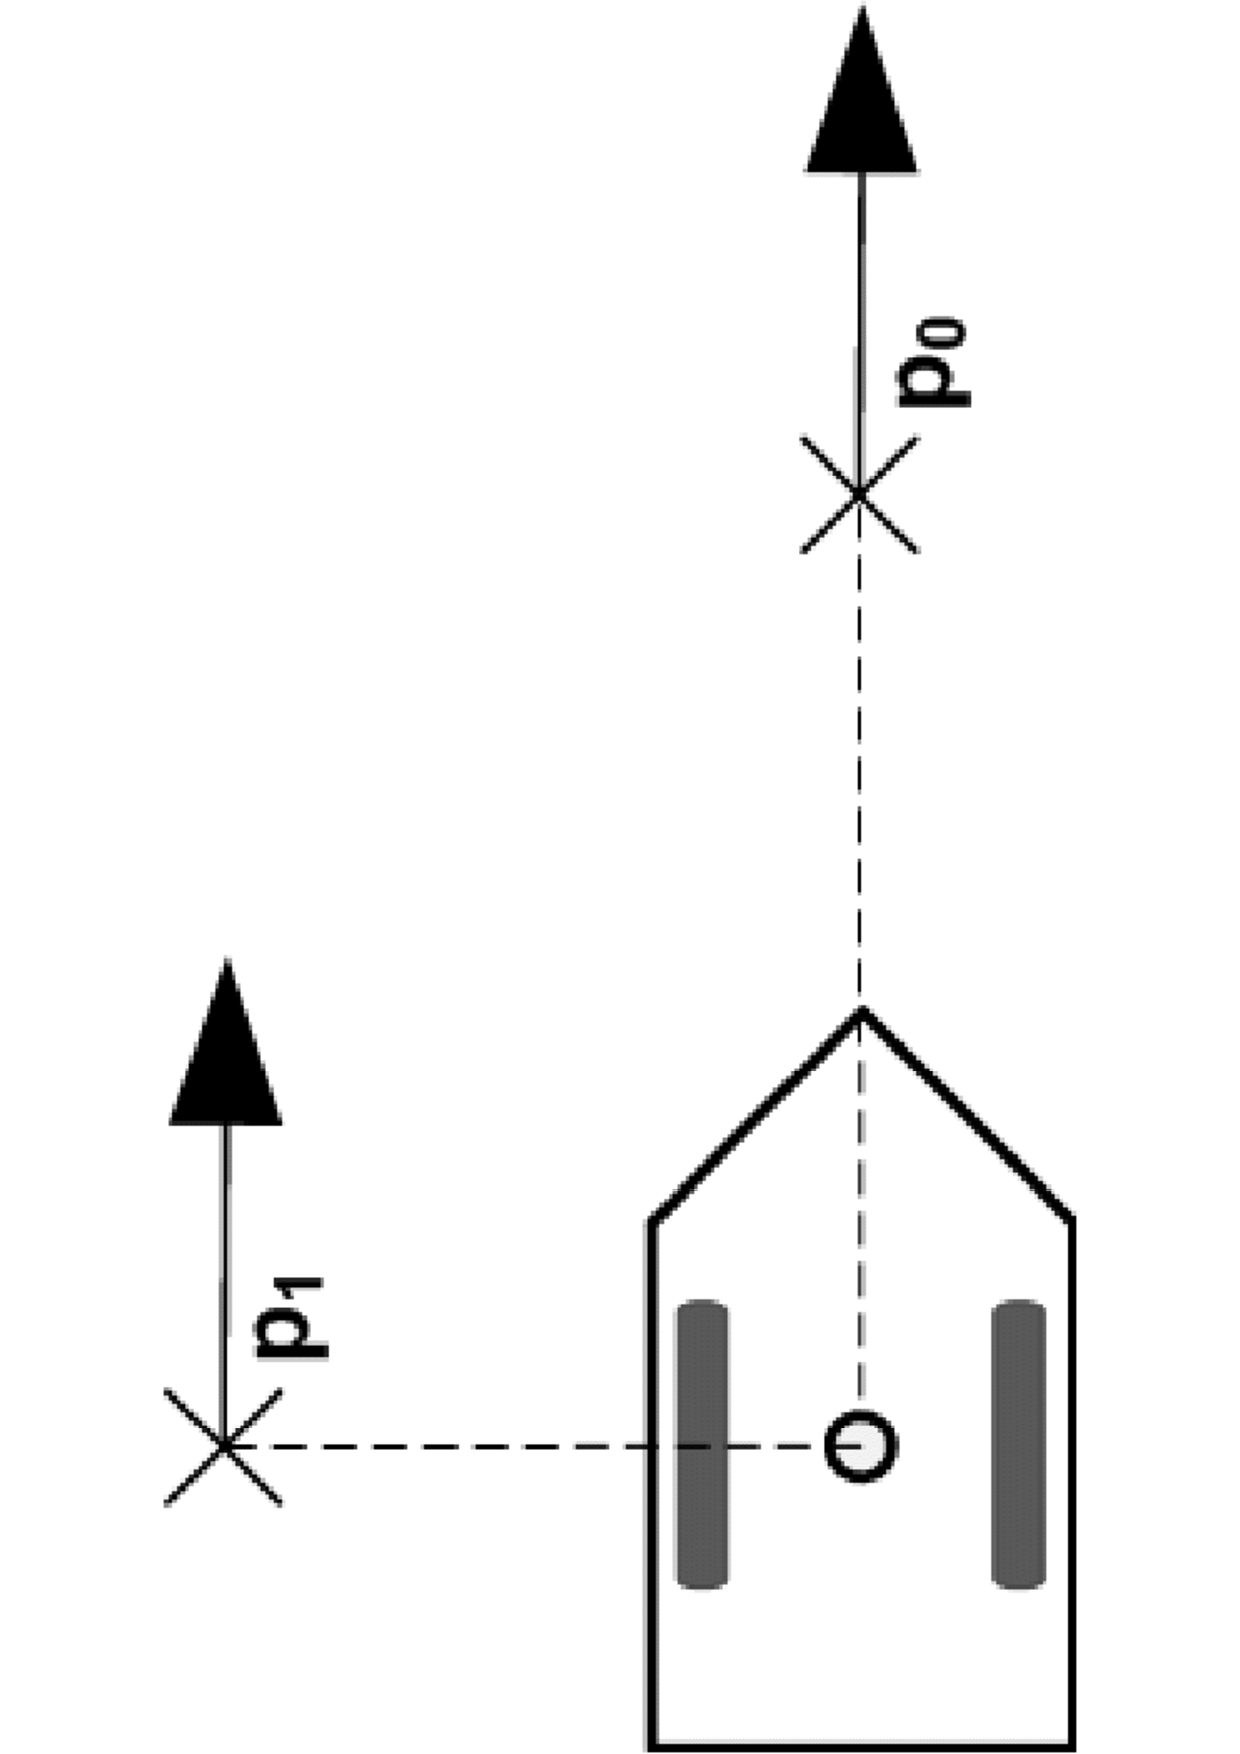
\includegraphics[scale=.2,angle=-90]{figures/rrtfunnel/non-holonomic-vehicle-euclidean-weakness}
  \caption{Consider two poses \(p_0\) and \(p_1\). Although \(p_1\) is nearer
    the robot in Euclidean distance it is harder to get to due to differential
    constraints. In this paper, we propose a directed distance function
    applicable to unicycle- type vehicles, that properly reflects the true
    cost-to-go of the system under the non-holonomic constraint. (figure
    courtesy of \cite{parkFeedbackMotionPlanning2015})}
  \label{fig:non-holonomic-vehicle-euclidean-weakness}
\end{figure}


\subsection{Funnel-Graph}

Look at ~\cite{vonasekGlobalMotionPlanning2013} (Algorithm3) for a way of
building an RRT with motion primitives.

\subsection{Funnel-graph}

Even though the \rrtfunnel{} algorithm can work just fine with a collection of
funnels, and simply brute-forcing all funnels at the planning stage, it is
helpful to associate some kind of structure with the collection. Therefore the
funnels will be organized into a graph structure \(\mathcal{F}\) where each
funnel is a edge in the graph, and the inlets and the outlets are vertices. The
funnels also need information about which funnels that they are composable with,
as they may not all be composable with each other, hence the graph is not
complete.

\begin{figure}
  \centering
  \begin{minipage}[b]{0.4\textwidth}
    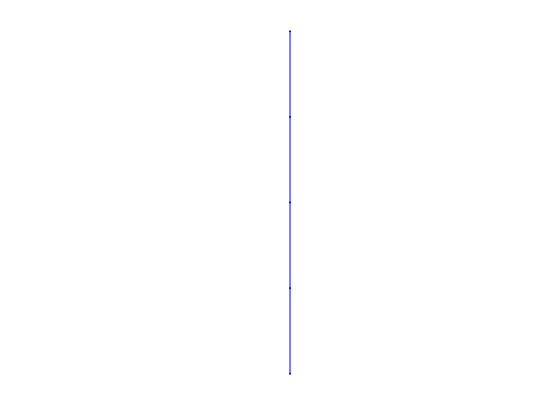
\includegraphics[width=\textwidth]{figures/method/trajectory-sampled}
    \caption{Trajectory sampled 21 times.}
  \end{minipage}
  \hfill
  \begin{minipage}[b]{0.4\textwidth}
    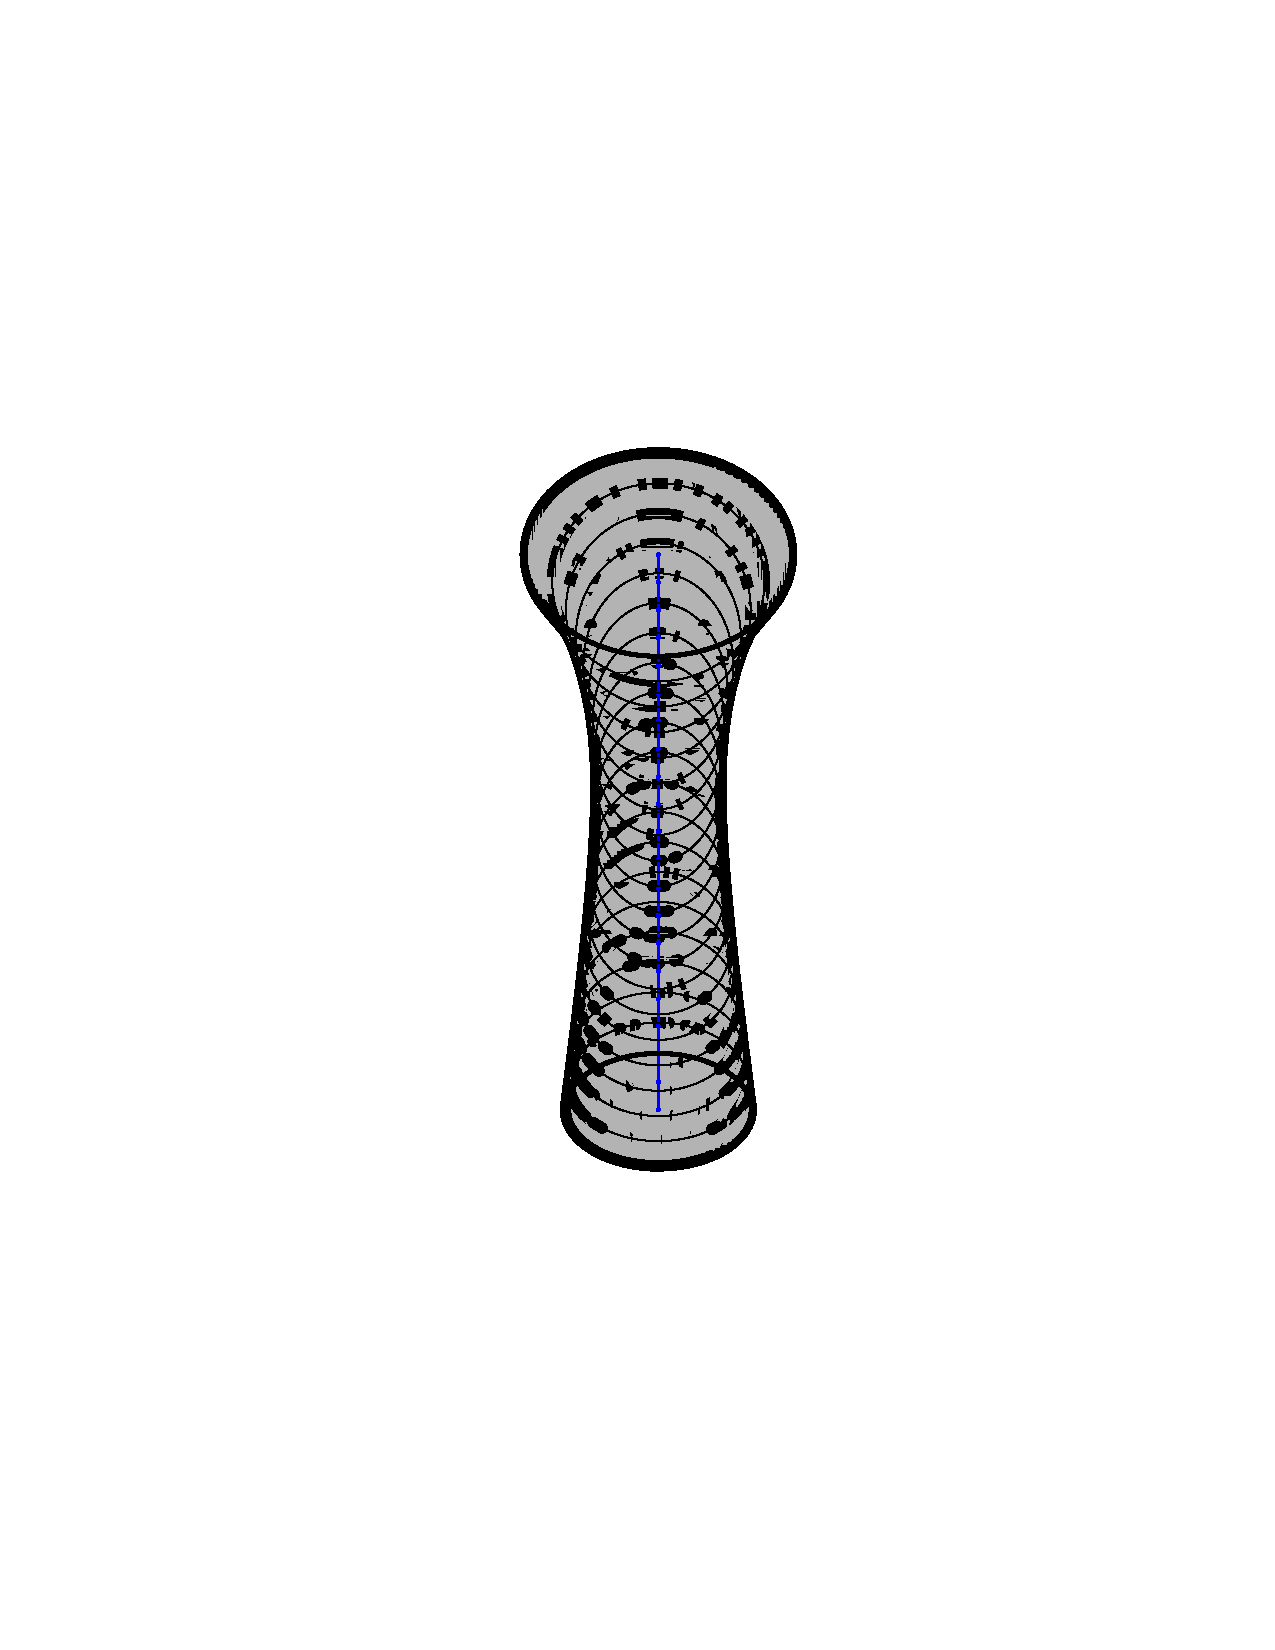
\includegraphics[width=\textwidth]{figures/method/funnel-sampled}
    \caption{The verified trajectory ellipsis overlaid at the sample times.}
  \end{minipage}
\end{figure}

For each funnel, in order to not only be able to compose funnels, but
sub-funnels, which means that at every point of every node in every funnel is
composable with every other sample point in every other funnel has to be
checked. This is summed up more orderly in algorithm
\cref{alg:create-funnel-graph}, where a funnel is a vertex in the graph, and an
ordered pair of funnels \(\left( F_{i}, F_{j} \right)\) is an edge. Composition
of funnels is checked in the same way as in \cref{def:funnel-composition}, and a
\ac{SOS}-program which implements the algorithm can be found in
~\cref{sec:funnel-composability-program-sos}.

\begin{algorithm}
  \caption{Create Funnel Graph}
  \label{alg:create-funnel-graph}
  \DontPrintSemicolon \SetAlgoNoLine

  \KwIn{\(\mathcal{F}\) -- The basis set of funnels computed around the nominal
    trajectories.} \KwOut{\(\mathcal{G}(\mathcal{F})\) -- Directed graph
    representing the composability of funnels.}

  \ForEach{\(F_{i} \in \mathcal{F}\)} { \ForEach{\(F_{j} \in \mathcal{F}\)} {
      \ForEach{\(t_{k} \in F_{i}\)} { \ForEach{\(t_{l} \in F_{j}\)} {
          \If{\(F_{i}(t_{k}) \subset F_{j}(t_{l})\)} { \(\mathcal{G}
            \leftarrow{} \left( F_{i}(t_{k}), F_{j}(t_{l}) \right)\) } } } } }

\end{algorithm}

\subsection{The \rrtfunnel{} algorithm}

With the framework finished, it is time to introduce the formulation of the
\rrtfunnel{} algorithm itself. The \rrtfunnel{} algorithm is a modified \ac{RRT}
algorithm which employs the precomputed funnels as motion primitives for its
expansion operator, and pseudocode for its definition can be found
in~\cref{alg:rrtfunnel}.

\begin{algorithm}
  \caption{Check funnel composability}
  \label{alg:create-funnel-graph}
  \DontPrintSemicolon \SetAlgoNoLine

  \KwIn{\(\mathcal{F}\) -- The basis set of funnels computed around the nominal
    trajectories.} \KwOut{\(\mathcal{G}(\mathcal{F})\) -- Directed graph
    representing the composability of funnels.}

  \ForEach{\(F_{i} \in \mathcal{F}\)} { \ForEach{\(F_{j} \in \mathcal{F}\)} {
      \If{\(F_{i}(t_{0}) \subset F_{j}(t_{end})\)} { \(\mathcal{G} \leftarrow{}
        \left( F_{i}(t_{0}), F_{j}(t_{end}) \right)\) } \; }\; }\;

\end{algorithm}

The \rrtfunnel{} algorithm is defined as

\begin{algorithm}[H]
  \caption{\rrtfunnel{} algorithm}
  \label{alg:rrtfunnel}
  \DontPrintSemicolon

  \KwIn{Initial configuration, \(q_0\)} \KwOut{\textit{RRT}-Funnel-graph
    \(\mathcal{G}\)}

  \SetKwFunction{RandConf}{Sample\_Random\_Configuration}
  \SetKwFunction{NearestVertex}{Find\_Nearest\_Vertex}
  \SetKwFunction{Extend}{Extend} \SetKwFunction{AddVertex}{add\_vertex}
  \SetKwFunction{AddEdge}{add\_edge}
  \SetKwFunction{ExtractBranch}{Extract\_Branch}
  \SetKwFunction{TestUncertainFunnels}{Test\_Uncertain\_Funnels}
  \SetKwFunction{BuildComposabilityMatrix}{Build\_Composability\_Matrix}

  Offline Phase: Generate the funnels

  Online Phase:

  \TestUncertainFunnels{} \; \BuildComposabilityMatrix{}

  \(\mathcal{G}.init(q_0)\) \For{\(i \leftarrow 1\) \KwTo \(k\)}{ \(q_{rand}
    \leftarrow \) \RandConf{} \; \(q_{near} \leftarrow \)
    \NearestVertex{\(q_{rand}, \mathcal{G}\)}\; \(q_{new} \leftarrow \)
    \Extend{\(q_{near}, q_{rand} \)}\; \If{\(q_{new} \in
      \modelconfigurationspacefree{} \) } {
      \(\mathcal{G}\).\AddVertex{\(q_{new}\)}\;
      \(\mathcal{G}\).\AddEdge{\(q_{near}, q_{new}\)} \; \If{\(q_{new} \in
        \mathcal{X}_{goal}\)}{ return \ExtractBranch{\(\mathcal{G}\)} \; }\; } }

  \SetKwProg{Def}{def}{:}{end} \Def{\RandConf{}}{ return 0\; }
  \Def{\TestUncertainFunnels{}}{ return 0\; } \Def{\BuildComposabilityMatrix{}}{
    return 0\; } \Def{\NearestVertex{\(q_{rand}, \mathcal{G}\)}}{ return 0\; }
  \Def{\Extend{\(q_{near}, q_{rand} \)}}{ return 0\; }

  \Def{\ExtractBranch{}}{ return 0\; }

\end{algorithm}

\subsection{Special maneuvers}

The algorithm incorporates room for two special maneuvers.

\subsubsection{The identity funnel for starting the simulation fresh}

The identity funnel is an empty placeholder for the start node of the graph,
that does no transformations on the model at all, and thus can be seen as the
identity element in the funnel space, or rather, the identity funnel.

\subsubsection{Emergency maneuver}

If the vehicle is to leave the verified funnel at execution time -- this could
happen for any number of reasons, such as unmodelled uncertainties -- the
vehicle should execute the emergency maneuver, which in this case is a simple
stop maneuver. Since the model employed is a simple first order model, a halt
will happen momentarily. Still, an emergency maneuver can be any sort of 'safe'
maneuver for the model at hand -- such as a loiter circle for an airplane, or
idling at one place for a quad-copter.

\subsection{Collision checking}
